\cotefile{57}
\scanpage{133}
% archive foliation: 132
\margin{$\ast$}
\uline{Théorème} Soit \deleted{$\unsure{Y'}\longleftarrow\unsure{X'}$}\inserted{$f:X\to Y$} un morphisme \uline{surjectif} de préschémas propres sur un corps $k$. Alors le noyau $\uuline{N}$ de $\uuline{\mathrm{Pic}}_{\unsure{Y}/k}\longrightarrow\uuline{\mathrm{Pic}}_{X/k}$ est \deleted{contenu} un sous-groupe d'un \uline{groupe affine} $G$ sur $k$.
\margin{?}

\unsure{Donc}

\uline{Corollaire}. Si $\uline{\mathrm{Pic}}_{Y/k}$ et $\uline{\mathrm{Pic}}_{X/k}$ existent, le noyau de $\uline{\mathrm{Pic}}_{Y/k}\mathbin{\text{---}}\uline{\mathrm{Pic}}_{X/k}$ est un groupe alg.-affine.

\uline{Corollaire} Dans les conditions précédentes, $\unsure{\mathrm{Nér\,Sév}}_{0}(Y/\deleted{\unsure{k}}k)\mathbin{\text{---}}\unsure{\mathrm{Nér\,Sév}}_{0}(X/k)$ est \uline{injectif}, et si $A$ et $B$ sont les ``parties abéliennes'' de $\uline{\mathrm{Pic}}_{Y/k}$ et $\uline{\mathrm{Pic}}_{X/k}$ \inserted{[\unsure{définies} si $k$ est parfait]} alors $A\longrightarrow B$ a un noyau fini.

\uline{Dém} \deleted{$\uline{\mathrm{Pic}}_X\unsure{\longleftarrow}\uline{\mathrm{Pic}}_{\unsure{Y}}$}, On va pour simplifier admettre que tous les $\uuline{\mathrm{Pic}}$ envisagés sont représentables.

a) On peut supposer $k$ \uline{alg. clos} (\unsure{extension}? )

b) On aura un diagramme de \uuline{schémas} \unsure{sur $k$}
\diagram{\left.\begin{tikzcd}
\uline{\mathrm{Pic}}_{X/k} \arrow[d,dash] & \uline{\mathrm{Pic}}_{Y/\unsure{k}} \arrow[l] \arrow[d,"\uline{\text{Aff.}}"] \\
\uline{\mathrm{Pic}}_{X_{\mathrm{réd}}} & \uline{\mathrm{Pic}}_{Y_{\mathrm{réd}}} \arrow[l,"?"]
\end{tikzcd}\right]\mathbin{\text{---}}\unsure{\text{ont}}}
\scanpage{134}
% archive foliation: 133
\[
\uline{f}^{m-n}:K_*(\uline{f}^{m})\qquad K_*(\uline{f}^{n})
\]
ou $m$ et $n$ sont des entiers rationnels, $m\quad n\quad0$, d'ou des \deleted{\unsure{en}}homomorphismes, notes par le meme symbole:
\[
K^*(\uline{f}^{n},M)\qquad K^*(\uline{f}^{m},M)
\]
et
\[
H^*(\uline{f}^{n},M)\qquad H^*(\uline{f}^{m},M)\qquad(m\quad n\quad0).
\]
Comme ces homomorphismes sont transitifs, on peut passer a la limite inductive dans ces homomorphismes, et poser
\[
C^*((\uline{f}^{\unsure{n}}),M)=\lim_n K^*(\uline{f}^{n},M)
\]
\[
\uline{H}^*((\uline{f}^{\unsure{n}}),M)\deleted{\unsure{*}}=H^*(C^*((\uline{f}),M)=\lim_n H^*(\uline{f}^{n},M).
\]
(N.B. dans ces notations, $(\uline{f})$ designe en fait l'ideal engendre dans $A$ par les $f_i$; on verra en effet ulterieurement que les objets introduits, \deleted{ne dependent} du moins $H^*((\uline{f}),M)$, ne depend que de cet ideal, et meme seulement de la topologie $\uline{m}$-adique qu'il definit, et non des $f_i$ eux-memes\unsure{.)}

Bien entendu, $C^*((\uline{f}),M)$ est un foncteur \deleted{exact} ($A$-lineaire exact) en $M$ et $H^*((\uline{f}),M)$ est un foncteur cohomologique en $M$.

Soit $\uline{f}$ comme ci-dessus, \deleted{\unsure{soit}} considere comme element du dual de $A^n$, soit $\uline{g}=(g_i)_{1\quad i\quad n}$ un element de $A^n$ lui-meme, on sait qu'on a alors, en designant par $e_{\uline{g}}$ l'operation de multiplication exterieure par $\uline{g}$ dans $A^n$, la \uline{formule d'homotopie}
\[
i_{\uline{f}}e_{\uline{g}}+e_{\uline{g}}i_{\uline{f}}=\langle\uline{g},\uline{f}\rangle\mathrm{id}.
\]
dans $\unsure{\Lambda}^{n}$, qui peut aussi s'ecrire, dans le complexe $K_*(\uline{f})$, comme
\[
de_{\uline{g}}+e_{\uline{g}}d=\uline{g},\uline{f}\quad\mathrm{id}.
\]
On en conclut la

\uline{Proposition 1}. Supposons que l'ideal $(\uline{f})$ engendre par les $f_i$ soit $A$. \unsure{Alors} le complexe $K_*(\uline{f})$ est homotopiquement equivalent a zero, et il en est \unsure{par} suite dememe des complexes $K_*(\uline{f},M)$ et $K^*(\uline{f},M)$ quels que soit $M$.
\margin{\unsure{Autre corollaire}: les $f_i$ annulent les $H_{\unsure{*}}(\uline{f},M)$, $H^{\unsure{*}}(\uline{f},M)$.}

\uline{Corollaire} S'il en est ainsi, on a $H^*(\uline{f},M)=0$ et $H^*((\uline{f}),M)=0$ pour \unsure{tout} $A$-module $M$.

Dans la description de $K^*(\uline{f},M)$, il faut aussi ajouter l'\unsure{interpretation} des elements de degre $p$ de ce complexe comme des fonctions alternees de $p$ indices variables entre $1$ et $n$; la formule du cobord est alors formellement celle d'un cobord en cohomologie de Cech.

2. \uline{Cohomologie de Cech d'un recouvrement ouvert}.

Soient $X$ un preschema, $A=\unsure{I|\Gamma}(X,\uline{O}_X)$, $\uline{f}=(f_i)_{1\quad i\quad n}$ un systeme de $n$ elements de $A$, $U_i=X_{f_i}$, $U=\quad U_i$, $\uline{U}$ le recouvrement de $U$ par les $U_i$. Soit $F$ un faisceau quasi-coherent sur $X$, posons
\[
M=\unsure{I|\Gamma}(X,F)
\]
(N.B. les notations precedentes devraient etre deployees de meme !)

\scanpage{135}
% archive foliation: 134
\deleted{\unsure{d)} Considérons donc la factorisation de Stein.}
\diagram{f\quad\left[\begin{tikzcd}X\arrow[r]&\unsure{Y'}\arrow[r,dash]&\unsure{Y}\end{tikzcd}\right]\unsure{\downarrow}}

On est ramené au cas où $Y$ est \uline{réduit}.

c) Prenons la factorisation de Stein
\diagram{\begin{tikzcd}X\arrow[r,dash]&Y'\arrow[r,dash]&\unsure{Y}\end{tikzcd}}
où $Y'\mathbin{\text{---}}Y$ est fini surjectif, donc un épimorphisme fini factorisable en produit d'épimorphismes stricts. Par ``\unsure{Sorb. chev.}'', $\uline{\mathrm{Pic}}_Y\mathbin{\text{---}}\uline{\mathrm{Pic}}_{Y'}$ est affine. On est ramené

\deleted{à prouver que $\uline{\mathrm{Pic}}_{Y'}\longrightarrow\uline{\mathrm{Pic}}_X$ l'est, \unsure{ce qui}}

\figure{\begin{tikzpicture}\draw[dashed] (0,0)--(12,0);\end{tikzpicture}}

ce qui nous ramène au cas $f_*(O_X)\simeq O_Y$.

d) Mais dans ce cas \unsure{on sait aussi que} $\uline{\mathrm{Pic}}_X\mathbin{\text{---}}\uline{\mathrm{Pic}}_Y$ est un mono, donc \unsure{de} \deleted{\unsure{noyau nul}} une immersion fermée, donc affine.

\margin{Attention au fait que $\uline{\mathrm{Pic}}_X$ et $\uline{\mathrm{Pic}}_Y$ ne sont pas de type fini sur $k$, \unsure{un mono n’est donc pas} néc\unsure{!} affine [ex. $\mathbf{Z}\to G$, $G=G_a$ ou bien VA]}

N.B. On s'est servi de l'existence des $\uline{\mathrm{Pic}}_Z$ pour $Z=Y_{\mathrm{réd}},X_{\mathrm{réd}}$, et pour les préschémas finis sur $Y_{\mathrm{réd}}$; \deleted{\unsure{Et}} on peut sans doute s'en passer !

\scanpage{136}
% archive foliation: 135
La codim coh de $M$ sur $B$ est celle de $\bar M$ sur $\bar B$. On en déduit: sous les conditions de cor.2, la codim. coh. de $M$ sur $B$ est identique à celle de $\bar M$ sur $\bar A$ (l'énoncer en corollaire; je m'aperçois que le cor.3 précédent devrait s'énoncer ainsi, avec : par conséquent $\dim_B M\quad\dim A$). On dit qu'un module de type fini sur un anneau local noethérien est Coh Mac si sa dim est égale à sa codim coh d'où un certain nombre de conséquences du lemme (qu'on peut donner en corollaires): Coh. Mac. est invariant par complétion, par changement fini d'anneau, enfin sous les conditions du cor.2 précédent \deleted{\unsure{xx}}, $M$ est Coh Mac sur $B$ si et seulement si $\bar M$ l'est sur $\bar A$. Enfin rappeler que si l'anneau local est régulier, Cohen Mac sur lui signifie libre. En fait, il faudrait sans doute un lemme spécial pour les Coh. Mac, en tous points parallèle (avec ses corollaires) au lemme sur la cocodim, mais contenant en plus le coup du régulier, et peut-être (pour avoir tout ensemble) l'équidimensionnalité. Pour l'instant, il n'était guère question de platitude dans ce numéro, mais:

\uline{Proposition} Soient $A\quad B$, \deleted{\unsure{M comme}\illegible{3}} un hom local d'anneaux locaux noethériens, $M$ un $B$-module de type fini. Pour que $M$ soit $A$-plat, il faut et il suffit que $\bar M$ (le complété du $B$-module $M$ pour sa topologie naturelle) soit plat sur $\bar A$.

Il faut évidemment noter que $\bar M$ (qui n'est pas en général le complété $\uline{m}$-adique de $A$, puisqu'onne fait pas d'hypothèse quasi-finie) est cependant un module sur $\bar A$. -- Démonstration: On applique le critère de prop.13, en notant que $\operatorname{Tor}_1^A(\uline{k},M)$ est un $B$-module de type fini, et que son complété est $\operatorname{Tor}_1^{\bar A}(\uline{k},\bar M)$.

\uline{Corollaire 1} Supposons de plus $M$ qu f sur $A$. Alors $M$ plat sur $A$ équivaut à $\bar M$ libre sur $\bar A$.

\uline{Corollaire 2} Supposons $M$ comme dans le cor.1 et $A$-plat, $\ne0$. Alors
\[
\dim_B M=\dim A\qquad \operatorname{cocodim}_B M=\operatorname{cocodim}_{\deleted{\unsure{\bar A}}}\bar A
\]
En effet, dim et cocodim sont invariants par complétion, d'autre part par changement raisonnable d'anneau, ce qui nous ramène d'abord au cas où $B$ lui-même\unsure{x} est qu f sur $A$, puis par complétion au cas où $A$ et $B$ complets (donc $B$ fini sur $A$) puis encore au\deleted{\unsure{cas}} $A=B$, enfin on note que la dim -- cocodim d'une somme directe est le sup resp. inf des dim \unsure{re}

\scanpage{138}
% archive foliation: 137
Soit $f:X\mathbin{\text{---}}S$ un morphisme se factorisant en
\diagram{\begin{tikzcd}X\arrow[r,dash,"\varphi"]&\Sigma\arrow[r,dash,"\psi"]&S\end{tikzcd}}
, avec $\psi$ fini, et $\varphi$ tel que $\uline{O}_{\Sigma}\simeq\varphi_*(O_X)$.

1) Alors on a
\diagram{\begin{tikzcd}\bullet\arrow[r]&\mathrm{Pic}(\Sigma)\arrow[r,dash]&\mathrm{Pic}(X)\arrow[r,dash]&\mathrm{Pic}'(X/S)\end{tikzcd}}
[suite exacte provenant de la suite spectrale de Leray].

\deleted{\unsure{et}} \uline{Si} $X/\Sigma$ admet une section, le dernier hom est un isom, i.e. dans ce cas
\[
\mathrm{Pic}'(X/S)\simeq\mathrm{Pic}(\unsure{X})/\mathrm{Pic}(\Sigma)
\]

Ce dernier fait se voit ainsi: \deleted{\unsure{Pour}} Soit $g:\Sigma\longrightarrow X$ une section de $X/\Sigma$; alors

i) \deleted{\unsure{pour}}\inserted{un} Module inversible $g$-rigidifié sur $X$ n'a pas d'aut. non trivial, ii) Tout Module inversible $\uline{L}$ sur $X$ est \deleted{\unsure{de norme}} $\mathrm{Pic}'(X/S)$ \uline{équivalent} à \deleted{l'image} un Module inversible $g$-rigidifié \inserted{[savoir $\uline{L}\otimes\varphi^*(g^*(\uline{L}))$]} [déterminé à isom unique près].

[On utilise le fait que $\mathrm{Pic}'(\Sigma/S)=0$].

On suppose pour la suite $f$ qu. cpt et qu. sép

\scanpage{139}
% archive foliation: 138
\margin{$\unsure{\simeq}$}
\diagram{\begin{tikzcd}[row sep=small,column sep=small]
&S\\
\Sigma\arrow[ur]&\\
&X\arrow[uu]\arrow[ul]
\end{tikzcd}}
% The following cancelled block is upside down on the supplied scan.
\diagram{\begin{tikzcd}
\deleted{X}\arrow[r,phantom,"{\underset{i}{\supset}}" description]\arrow[d,"\deleted{f}"']&\deleted{Z}\arrow[dl,"\deleted{\varphi}"]\arrow[r,phantom,"\deleted{\text{fermé}}"]&{}\\
\deleted{S}&&
\end{tikzcd}}
\deleted{Supposons}

\deleted{i) $Z$ fini sur $S$}

\deleted{ii) $f_*(O_X)\xrightarrow{\sim}\varphi_*(O_{\unsure{S}})$}

\deleted{Alors (i) Tout Module inversible sur $X$ est $\mathrm{Pic}'(X/S)$-équivalent à un Module}

\scanpage{140}
% archive foliation: 139
2) Soit $S'\mathbin{\text{---}}S$ fid. plt et qu. cpt. Alors

i)
\[
\mathrm{Pic}'(X/S)\mathbin{\text{---}}\mathrm{Pic}'(X'/S')
\]
est injectif. ii) Si $X/\Sigma$ a \deleted{\unsure{une}} une section \deleted{sur} localement sur $S$, alors
\diagram{\begin{tikzcd}
\mathrm{Pic}'(X/S)\arrow[r]&\mathrm{Pic}'(X'/S')\arrow[r,shift left]\arrow[r,shift right]&\mathrm{Pic}'(X''/S'')
\end{tikzcd}}
est exact.
\margin{généraliser à des familles \unsure{recouvrantes} du type $\unsure{U^*}$ dès l'abord \unsure{---}}

On peut dém. (i) partant d'un $\uline{L}$ inv. sur $X$. \inserted{En vertu de 1)} L'hyp. signifie que $\uline{L}'$ provient de $\Sigma'$. Or $\Sigma'$ est fid. plt qu. cpt sur $\Sigma$. On sait que alors $\uline{L}$ provient de $\Sigma$.

Pour (ii), \inserted{grâce à (i)} la question est locale sur $S$, on peut donc supposer que $X$ a une section sur $\Sigma$. Alors on utilise le théorème de descente connu et le raisonnement connu.

\uline{Corollaire} \deleted{\unsure{1}} Dans les conditions précédentes, $\mathrm{Pic}'(X/S)\longrightarrow\mathrm{Pic}^{\unsure{\sharp|*}}(X/S)$ est injectif, et est bijectif si $X/\Sigma$ \deleted{\unsure{localement}} a une section loc. sur $S$.

Si $X/\Sigma$ a \unsure{=} une section, on a un isom
\[
\mathrm{Pic}(X/S)\simeq\mathrm{Pic}(X)/\mathrm{Pic}(\Sigma)
\]

\scanpage{141}
% archive foliation: 140
Picard des schémas \unsure{en} courbes

\scanpage{142}
% archive foliation: 141
$f:X\longrightarrow S$ projectif et lisse, fibres géom connexes de dim 1.

$U=X-Y$, \inserted{p. ex. $Y=$} $[\coprod_{i\in I}g_i(S)$, les $g_i$ des sections telles que les $g_i(S)$ deux à deux disjoints$]$
\margin{$Y$ sous-schéma fermé de $X$ \uline{étale} sur $S$}
\[
f_U:U\mathbin{\text{---}}S
\]
$n$ premier aux car. résiduelles\inserted{ de $S$}. On trouve
\[
E_2^{pq}=H^p(S,\underbrace{R^q_!f_U(\mu_n)}_{\substack{0\text{ sauf si}\\q=1,2}})\Longrightarrow H^*_{\mathrm{prop}}(\unsure{U},\mu_n)
\]
\[
R^q_!f_U(\mu_n)=\begin{cases}
0&\text{si }q\unsure{\notin|\ne}\{1,2\\
{}_n\mathbf E&\text{si }q=1\\
(\mathbf Z/n\mathbf Z)_S&\text{si }q=2
\end{cases}
\]
\margin{(def. de $E$ cf plus bas)}
\figure{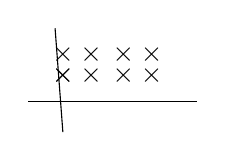
\begin{tikzpicture}[scale=.55]
\draw (-.8,0)--(3.1,0);\draw (0,-.7)--(-.18,1.7);
\foreach \x in {0,.65,1.4,2.05}{\node at (\x,.6) {$\times$};\node at (\x,1.1) {$\times$};}
\node[font=\bfseries] at (0,.6) {$\times$};
\end{tikzpicture}}
\diagram{\begin{tikzcd}
E_2^{02}\arrow[r]\arrow[d,equal]&E_2^{2,1}\arrow[d,equal]\\
H^0(S,\mathbf Z/n\mathbf Z)&H^2(S,{}_n E)
\end{tikzcd}}

On trouve un élément canonique
\[
\xi_n\in H^2(S,{}_n E)
\]
Si $n=\ell^\nu$ ($\nu$ variable), $\ell$ premier distinct des car. rés. sur $S$, on trouve
\[
\boxed{\xi(\ell)\in H^2(S,\mathbf T_\ell(E))}
\]
Cet \uline{élément est nul si} $U$ \uline{a une section sur} $S$.

$\mathbf E$ est un schéma en groupes lisse sur $S$, \deleted{\unsure{et}}\inserted{à fibres connexes}, (extension de $J=\uline{\mathrm{Pic}}^0_{X/S}$ par $T=G_m^I/G_m$\inserted{ $\longrightarrow$ diagonale})
\diagram{\begin{tikzcd}
0\arrow[r]&T\arrow[r]\arrow[d,equal]&\mathbf E\arrow[r]&J\arrow[r]&0\\
&G_{mS}^I/G_{mS}&&&
\end{tikzcd}}

\scanpage{143}
% archive foliation: 142
% The typescript is upside down in the supplied scan; reading order follows the letter.
INSTITUT

DES HAUTES ÉTUDES SCIENTIFIQUES

91 - BURES-SUR-YVETTE

928-48-53

Massy November 21, 1966

Dear Mr Benjamin,

I got the front matter for the book ``Huit exposés ... '', which I am now sending back to you with two minor corrections. A more serious matter - and this is why I am adressing this letter to you rather than to Miss Ball - is the interrogation mark on page three concerning the mention ``Copyright 1966 by W.A. Benjamin, Inc ''. In your letter of july 8 1966, you stated that the copyright would remain with Mr Bourbaki, and I have been assuming till now that the book was being published under this proviso. If you should have changed your mind about it, I will have to check with Bourbaki if it is all right with him, which (whatever his decision) will cause a delay of a few months more. Once this matter set straight, everything is all right with me resp. the front matter, and you can go ahead$_x$ with the printing. I would only like to know if you got \unsure{my} letter of November 10 proposing to include still another paper, and your opinion about this suggestion.

Sincerely yours

\figure{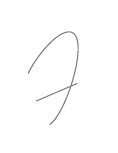
\begin{tikzpicture}[scale=.5]
\draw[gray] (0,0) .. controls (.45,.35) and (1,2.2) .. (.55,2.35) .. controls (.2,2.45) and (-.4,1.65) .. (-.55,1.3);
\draw[gray] (-.35,.6)--(.7,1.05);
\end{tikzpicture}}

\scanpage{144}
% archive foliation: 143
On obtient $E$ ainsi: \deleted{\unsure{collapsant $Y$|collapse $Y$}} On définit un schéma en courbes plat $Z$ sur $S$ comme conoyau de
\diagram{\begin{tikzcd}
X\amalg(Y\times_S Y)\arrow[r,shift left,"{\mathrm{id}_X,\alpha\operatorname{pr}_1^{Y/S}}"]\arrow[r,shift right,"{(\mathrm{id}_X,\alpha\operatorname{pr}_2^{Y/S})}"']&X
\end{tikzcd}\qquad(\alpha:Y\hookrightarrow X)}
et on définit
\[
\mathbf E=\uline{\mathrm{Pic}}^0_{Z/S}.
\]
\deleted{\unsure{Morphisme}} Le morphisme $\mathbf E\longrightarrow J$ est induit par $X\xrightarrow{\varphi}Z$ en passant aux $\uline{\mathrm{Pic}}^0_{/S}$. Notons que nous avons un torseur canonique $P$ sous $E$,
\[
P=\uline{\mathrm{Pic}}^1_{Z/S}
\]
(et, d'ailleurs, un $S$-morphisme can $U\longrightarrow P$).

Notons que $P$ définit un élément
\[
\boxed{\eta\in H^1(S,E)},
\]
et la relation entre $\xi_n$ et $\eta$ est
\[
\boxed{\xi_n=\delta_n(\eta)},
\]
\margin{à vérifier ......}
où $\delta_n$ est l'opérateur cobord
\[
H^1(S,E)\mathbin{\text{---}}H^2(S,{}_n E)
\]
associé à la suite exacte de Kummer
\diagram{\begin{tikzcd}
0\arrow[r,dash]&{}_n E\arrow[r,dash]&E\arrow[r,dash,"n\mathrm{id}_E"]&E\arrow[r,dash]&0.
\end{tikzcd}}

\scanpage{145}
% archive foliation: 144
Notons que l'image de $\eta$ dans $H^1(S,J)$, par fonctorialité, n'est autre que la classe de $\uline{\mathrm{Pic}}^1_{X/S}$ (considéré comme torseur sous $J$). Supposons cette classe nulle [ce qui est le cas si $X/S$ admet une section]. \deleted{p. ex.} Alors la suite exacte
\diagram{\begin{tikzcd}
H^0(S,J)\arrow[r]&H^1(S,T)\arrow[r,dash]&H^1(S,E)\arrow[r,dash]&H^1(S,J)
\end{tikzcd}}
montre que \deleted{$\unsure{\eta}$} $\eta$ est dans $\operatorname{Im}H^1(S,T)$.

Notons qu'on a d'ailleurs une suite exacte \inserted{(si $Y\mathbin{\text{---}}S$ surjectif)}
\diagram{(*)\quad\begin{tikzcd}
0\arrow[r]&G_{mS}\arrow[r]&\prod_{Y/S}G_m\arrow[r]&T\arrow[r,dash]&0
\end{tikzcd}}
qui donne une suite exacte \deleted{\unsure{longue}}
\diagram{\begin{tikzcd}[column sep=small]
\unsure{0}\arrow[r]&H^0(S,O_S)^*\arrow[r,dash]&H^0(Y,O_Y)^*\arrow[r,dash]&H^0(S,T)\arrow[r,dash]&\mathrm{Pic}(S)\arrow[r]&\mathrm{Pic}(Y)\arrow[r,dash]&H^1(S,T)\arrow[r]&\mathrm{Br}'(S)\arrow[r]&\mathrm{Br}'(Y),
\end{tikzcd}}

Lorsque la suite exacte est splittée, p. ex. lorsque $Y$ admet une section sur $S$, alors on trouve
\[
\deleted{H^1(S,T)\unsure{\simeq}}\qquad H^1(S,T)\simeq\mathrm{Pic}(Y)/\operatorname{Im}\mathrm{Pic}(S)
\]
et lorsque $Y=\coprod_{i\in I}g_i(S)$ comme dessus, alors
\[
\deleted{\unsure{on trouve}}\qquad\mathrm{Pic}(Y)\simeq\mathrm{Pic}(S)^I
\]
et on trouve
\[
H^1(S,T)\simeq\mathrm{Pic}(S)^I/\operatorname{Im}\mathrm{Pic}(\unsure{S})
\]
\inserted{$\longrightarrow$ par diagonale.}

Si p. ex. $\mathrm{Pic}(S)=0$, on trouve $\eta=0$, à fortiori les $\xi_n$, $\xi_\ell$ sont nuls.

\scanpage{147}
% archive foliation: 146
Soit $C$ une courbe complète, réduite et connexe sur $k$\inserted{alg. clos}.
On veut calculer $\mathrm{Pic}_C$
\diagram{\begin{tikzcd}
0\arrow[r,dash]&\uline{O}_C^*\arrow[r,dash]&\widetilde{\uline{O}}_C^*\arrow[r]&\prod_P A_P^*\arrow[r,dash]&0
\end{tikzcd}\qquad P\ \text{les pts doubles}}
\diagram{\begin{tikzcd}[column sep=small,execute at end picture={
\draw[rounded corners=2pt] ([yshift=-3pt]\tikzcdmatrixname-1-2.south west) -- ++(0,-5pt) -| ([yshift=-3pt]\tikzcdmatrixname-1-4.south east);
\node[below=11pt] at (\tikzcdmatrixname-1-3.south) {$\unsure{G}$};
}]
0\arrow[r]&G_m\arrow[r,dash]&\prod_{C_i}G_m\arrow[r]&\prod_{P_\alpha}A_P\arrow[r]&\mathrm{Pic}_{C/k}\arrow[r]&\prod\mathrm{Pic}_{\widetilde C_i/k}\arrow[r]&0
\end{tikzcd}}
\figure{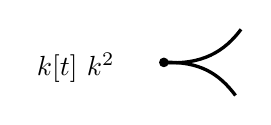
\begin{tikzpicture}[scale=.7]
\node at (-1.6,-.1) {$\unsure{k[t]}\ \unsure{k^2}$};
\fill (0,0) circle (2.5pt);
\draw[very thick] (0,0) .. controls (.7,-.05) and (1.1,.2) .. (1.4,.6);
\draw[very thick] (0,0) .. controls (.65,.02) and (1.0,-.2) .. (1.3,-.6);
\end{tikzpicture}}
On trouve que l'on a dans $\mathrm{Pic}_{\unsure{C^0/k|C/k}}$ une partie linéaire,
\deleted{\unsure{et un gr. multiplicatif}}, qui est isomorphe à
\[
G=\left(\prod_{P_\alpha}A_{P_\alpha}\right)/(\prod G_m/G_m)
\]
donc est de dimension égale à
\[
\dim G=\sum\mu_\alpha-c_0+1
\]
\margin{$c_0=\text{\unsure{nbr des composantes}}\ C_i$}
où $\mu_\alpha=\dim\unsure{A_\alpha|A_{P_\alpha}}$
\deleted{\unsure{\`a}\illegible{2}\ $P_\alpha$} \inserted{$=\dim_k\uline{O}_{\widetilde C}/\uline{O}_C$}.
\unsure{Posons}
\[
\unsure{\mu_\alpha}=1+\delta_\alpha,
\qquad\deleted{\text{\unsure{on trouve donc}}}
\]
\deleted{
\[
\dim G=c_1-c_0+1+\sum\delta_\alpha=b_1+\sum\delta_\alpha
\]
\deleted{\unsure{donc}}
où $b_1$ est le nbr de cycles du schém. combinatoire de $C$.
\margin{$c_0-c_1=1-b_1$}
La dimension de la partie \deleted{multiplicative}\inserted{additive} de $G$ est
\[
\deleted{\unsure{\sum_\alpha(d_\alpha-1)-(\sum d_\alpha)-c_1=2c_0-c_1=}}
\]
\[
\deleted{\unsure{\sum_\alpha(\mu'_\alpha-1)-c_0+1}}
\qquad\sum(\mu_\alpha-\mu'_\alpha)
\]
où $\mu'_\alpha$ est la multiplicité ``ensembliste'' de $P_\alpha$, $=$ nbr de
\deleted{\unsure{courbes}}\inserted{branches formelles} passant par $\alpha$.
}

\scanpage{148}
% archive foliation: 147
\begin{center}42\end{center}
let $D'_h=\widetilde\Phi^{-1}(D_h^{*\prime})$. Clearly $D_h^{*\prime}$ meets $D_h^*$ at simple intersection points only and therefore $(D_h^{*2})=(D_h^*D_h^{*\prime})$ is equal to the number of these intersection points, while each intersection point of $D_h^{*\prime}$ and $D_h^*$ corresponds to $m$ intersection points of $D'_h$ and $D_h$. Hence we have
\[
(D_h^2)=(D_hD'_h)\geqq m(D_h^{*2})=2mah^2,
\]
and therefore
\[
\dim|D_h|\geqq mah^2-bh+\chi(\widetilde V)-1-\widetilde p_g,
\]
where $2b=(KD_1)$ and $\widetilde p_g$ is the geometric genus of $\widetilde V$. Combined with the equality
\[
\dim|D_h|=\dim|D_h^*|=ah^2-b^*h+\chi(V*)-1,
\]
this proves that
\[
mah^2-bh\leqq ah^2-b^*h+\text{const.},\quad\text{for all }h\geqq1,
\]
where $a=\frac12(D_1^{*2})$ is positive. Consequently we obtain $m=1$.
Thus the inverse image $\widetilde\Phi^{-1}(\mathfrak p*)$ of the general point $\mathfrak p*$ on $V*$ consists of a single point and therefore $\widetilde\Phi^{-1}$ has no branch curve. Hence $\widetilde\Phi^{-1}$ is regular and single-valued except for a finite number of fundamental points. $\widetilde\Phi$ is therefore bi-regular on $\widetilde V$ except for a finite number of fundamental curves.

Now these fundamental curves can be eliminated by quadratic transformations. Namely, by applying a finite number of

\scanpage{149}
% archive foliation: 148
Posons
\[
\mu_\alpha=\mu'_\alpha+\mu''_\alpha
\]
$\mu'_\alpha$ partie multiplicative $=$ nbr de branches \uline{formelles} passant par $P_\alpha$, diminué de $1$

$\mu''_\alpha$ partie additive \deleted{\unsure{de}}.
\[
\dim G_{\mathrm{mult}}=\sum\mu'_\alpha-c_0+1=h_1
\]
\margin{\uline{\unsure{invariant topologique}} \uline{des 2 situations}}
[ N.B. Lorsque les $C_i$ \deleted{\unsure{peuvent avoir des}} pts multiples\deleted{\unsure{quelconques}}, alors $h_1$ \unsure{n'est} pas déterminé \deleted{\unsure{par}} combinatoirement par le schém.
\deleted{\unsure{de rencontre}}\inserted{combinatoire de $C$}. Il est en tous cas déterminé par le schém. combinatoire de la \unsure{descente} $\widetilde C\longrightarrow C$; il est aussi le rang du \deleted{$\unsure{\Pi}$} noyau de
$H^1_{\unsure{\ell}}(C)\longrightarrow\deleted{\unsure{\prod}}H^1(\widetilde C)$, (Cohomologie de Weil) ou du conoyau de
\[
\prod\pi_1(\widetilde C_i)-\pi_1(C)\ ]
\]
\[
\dim G_{\mathrm{add}}=\sum\mu''_\alpha
\]
Dire que $\mathrm{Pic}^0$ n'a que des composantes \deleted{\unsure{linéaires}} multiplicatives, signifie que les recollements en $P_\alpha$ sont \unsure{triédraux|triviaux}\inserted{formels; \unsure{Alors} $\mu_\alpha=\mu'_\alpha\geq2$}.
Dire que c'est une V.A. \deleted{signifie} \inserted{implique} que \deleted{\unsure{les}} de plus

\scanpage{150}
% archive foliation: 149
\begin{center}40\end{center}
Now let $V$ be a compact analytic surface with two algebraically independent meromorphic functions $x,y$. Then, by the result of Chow mentioned above, $\unsure{\mathfrak M|\mathcal M}(V)$ is a finite algebraic extension of the field $\mathbb C(x,y)$ of rational functions in $x,y$. (A proof of this fact based on our results in Section 1 will be given in Appendix below.) Hence there exists a \uuline{non-singular} \uline{algebraic surface} $V*$ in a projective space such that $\unsure{\mathfrak M|\mathcal M}(V)\cong\unsure{\mathfrak M|\mathcal M}(V*)$. Letting $(1,x_1^*,\ldots,x_d^*)$ be the \uline{generic} point of $V*$ and letting $x_k=x_k(z)$ be the meromorphic function on $V$ corresponding to $x_k^*$ by the isomorphism $\unsure{\mathfrak M|\mathcal M}(V)\cong\unsure{\mathfrak M|\mathcal M}(V*)$, we define a meromorphic mapping $\Phi$ of $V$ onto $V*$ by
\[
z\longrightarrow\Phi(z)=(1,x_1(z),\ldots,x_d(z)).
\]
This mapping $\Phi$ is regular on $V$ except for a finite number of its fundamental points. These fundamental points can be eliminated by means of quadratic transformations. Namely, by applying a finite number of suitable quadratic transformations $Q_{\mathfrak p},Q_{\mathfrak p'},Q_{\mathfrak p''},\ldots$ to $V$ successively, we obtain a compact analytic surface
\[
\widetilde V=\ldots.\ Q_{\mathfrak p''}Q_{\mathfrak p'}Q_{\mathfrak p}(V)
\]
such that the mapping $\widetilde\Phi=\Phi Q_{\mathfrak p}^{-1}Q_{\mathfrak p'}^{-1}Q_{\mathfrak p''}^{-1}\ldots$ of $\widetilde V$ onto $V*$ is everywhere regular.$^7$ Since $\Phi$ induces the isomorphism

\noindent\rule{.28\linewidth}{.4pt}

${}^7$ Chow and Kodaira, loc. cit., p. 322.

\scanpage{151}
% archive foliation: 150
\deleted{il faut \unsure{en effet}} les $C_i$ sont non singulières
[car $\unsure{\mathrm{Pic}_{C_i/k}^0}$ est un quotient de $\mathrm{Pic}_{C/k}^0$] et \deleted{\unsure{que}}
\deleted{\unsure{les} $\mu'_\alpha$ \unsure{est le nbr des} $C_i$ qui passent par \unsure{$P_\alpha$},}
pour $i\ne j$, alors $C_i$ et $C_j$ se coupent en un pt au plus
[car $\mathrm{Pic}(C_i\cup C_j)$ est un quotient de $\mathrm{Pic}(C)$].
\deleted{Soit $\nu_\alpha$ le nbr des $C_i$ passant par $P_\alpha$, on a
\[
\begin{aligned}
\dim G_{\mathrm{mult}}&=\sum(\nu_\alpha-1)-c_0+1\\
&=\sum_i(\text{nbr des pts }P_\alpha\text{ sur }C_i-1)-
\end{aligned}
\]
}
Alors finalement, on trouve de cette façon que l'on ne peut avoir de cycles
\figure{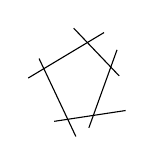
\begin{tikzpicture}[scale=.55]
\draw (-.35,.55)--(1.4,1.6); \draw (.7,1.7)--(1.75,.6);
\draw (1.7,1.2)--(1.05,-.6); \draw (1.9,-.2)--(.25,-.45);
\draw (-.1,1)--(.75,-.8);
\end{tikzpicture}}
dans le schém. combinatoire de $C$. \deleted{\unsure{(un arbre)},}
\unsure{Réciproqt}, si $C$ n'a que des pts \deleted{doubles}\inserted{multiples}
``multiplicatifs'', et si les $C_i$ sont non singuliers, on voit par récurrence sur le nb des $C_i$ que
\deleted{$C$} $\mathrm{Pic}_{C/k}^0$ \unsure{est} une V.A.

On aura en tous cas
\[
\begin{aligned}
g=\dim\mathrm{Pic}_{C/k}&=\sum g_i+(\sum_\alpha\mu_\alpha-c_0+1)\\
&=\sum g_i+\deleted{\unsure{h_1}}\rho+\sigma
\end{aligned}
\]
\margin{$g_i=\text{genre de }\widetilde C_i$}
$\rho=$ nb des cycles combinatoires, $+$ somme des \unsure{nbrs} des multiplicités multiplicatives des $C_i$
[\unsure{nulles donc} $=0$ si les $C_i$ non sing]

$\sigma=$ somme des multiplicités additives des $P_\alpha$.

\scanpage{152}
% archive foliation: 151
\begin{center}39\end{center}
regular map of $\widetilde V$ onto $V$ which is bi-regular between $\widetilde V-S$ and $V-\mathfrak p$. It is easy to prove the following propositions:$^4$

i) $Q_{\mathfrak p}^{-1}$ induces an isomorphism: $\unsure{\mathfrak M|\mathcal M}(Q_{\mathfrak p}(V))\cong\unsure{\mathfrak M|\mathcal M}(V)$.

ii) If $V$ is a non-singular algebraic surface in a projective space, then $Q_{\mathfrak p}(V)$ is also a non-singular algebraic surface in a projective space.

Moreover we have

\begin{quote}
CASTELNUOVO-ENRIQUES' THEOREM:$^5$ Let $\widetilde V$ be a non-singular algebraic surface in a projective space and let $S$ be a non-singular rational curve on $\widetilde V$ with $(S^2)=-1$. Then there exists a non-singular algebraic surface $V$ in a projective space and a point $\mathfrak p$ on $V$ such that $Q_{\mathfrak p}(V)=\widetilde V$ and $Q_{\mathfrak p}(\mathfrak p)=S$.
\end{quote}

The following proposition$^6$ is a corollary to this theorem:

iii) If $Q_{\mathfrak p}(V)$ is a non-singular algebraic surface in a projective space, then $V$ is also a non-singular algebraic surface in a projective space.

\noindent\rule{.28\linewidth}{.4pt}

${}^4$ See Chow and Kodaira, loc. cit.

${}^5$ G. Castelnuovo and F. Enriques, Sopra alcune questioni fondamentali nella teoria delle superficie algebriche, Annali di Math., Ser. III, Vol. 6 (1901), pp. 165--225, Chap. III. See also K. Kodaira, On Kähler varieties of restricted type, Annals of Math., Vol. 60 (1954), pp. 44--48.

${}^6$ Chow and Kodaira, loc. cit., Lemma 3.

\scanpage{153}
% archive foliation: 152
\figure{\begin{tikzpicture}[x=.65cm,y=.65cm]
\draw (0,6)--(2,8); \draw (.7,7.8)--(1.3,5.2); \draw (1.2,7.8)--(2.35,6.1);
\draw (.7,5.9)--(3.2,4.5); \draw (1.7,5.7)--(1.7,4.35); \draw (2.25,5.55)--(2.1,4.1);
\node at (3.5,4.5) {$g$};
\draw (-.1,2.3)--(1.15,4); \draw (.2,4.25)--(.55,1.7); \draw (.6,4.05)..controls (1.15,3.9)..(1.7,2.7);
\draw (.05,2.05)--(1.7,1.1); \draw (.7,2.1)--(1.3,.25); \draw (1.25,2.1)--(.9,.65); \fill (1.05,1.55) circle (2pt);
\draw (3,1)--(4.6,2.6); \draw (3.15,2.4)--(3.6,-.1); \draw (4,2.7)..controls (4.2,1.5)..(4.85,.7);
\draw (3.2,.6)--(5.8,-1.15); \draw (4.15,.25)--(4,-1); \draw (4.7,.05)--(4.5,-1.3); \draw (5.35,-.1)--(4.95,-2.65);
\node at (5.8,.05) {$g''$}; \node at (6.1,-1.2) {$g'$};
\node at (9,-.3) {$g'+g''=g\quad(g'+g''>0)$};
\draw (11,2)--(13,3.5); \draw (11.3,3.2)..controls (11.6,1.6)..(12.1,.9); \draw (12.65,3.65)..controls (12.9,2.7)..(13.5,2.05);
\draw (11.2,1.5)--(14.2,.65); \draw (11.45,1.85)--(11,.1);
\draw (12.55,1.6)--(12.5,.1); \draw (13.05,1.4)--(13,.0); \draw (13.55,1.2)--(13.65,-.2);
\node at (14.7,.65) {$\deleted{\unsure{g}}g'=0$}; \node at (17,.55) {$(g=0$};
\end{tikzpicture}}
\[
\sum_{g_i\unsure{\geq|>}1}(3g_i-3+\nu_i\deleted{\unsure{0}})
+\sum_{g_i=1}\underbrace{(1+\nu_i-1)}_{3g_i-3+\nu_i}
+\sum_{\substack{g_i=0\\\nu_i\unsure{>|\geq}3}}
\deleted{\text{\unsure{sauf les}\illegible{1}}}\underset{3g_i-3+\nu_i}{\nu_i-3}
\]
$\nu_i=$ nb des pts \deleted{\unsure{multiples}}\inserted{\unsure{marqués}} sur $C_i$
\[
3\sum g_i-3c_0+\sum\nu_i+\overset{\lambda}{\boxed{\sum_{\substack{g_i=0\\\nu_i\leq2}}3-\nu_i}}
\]
$\lambda=$ nb des courbes $C_i$ de genre $0$, avec $\nu_i=2$ (\unsure{minimum})
\figure{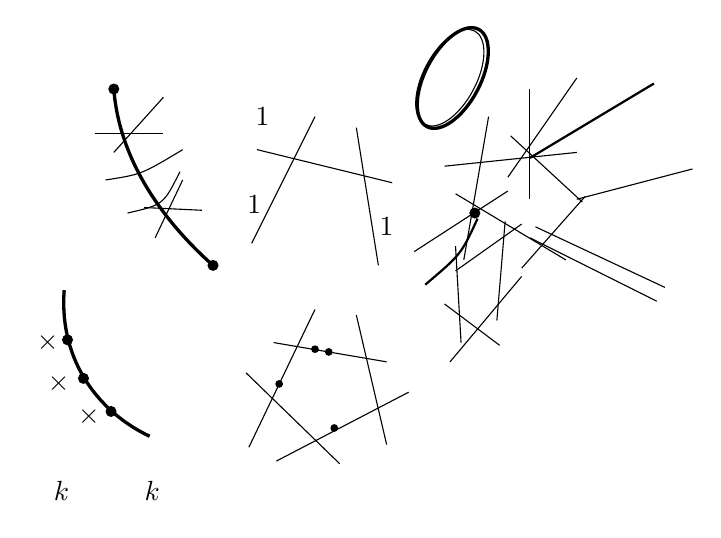
\begin{tikzpicture}[x=.7cm,y=.7cm]
\draw[very thick] (0,6)..controls (.1,4.7) and (.9,3.6)..(1.8,2.8); \fill (0,6) circle (2pt); \fill (1.8,2.8) circle (2pt);
\draw (-.35,5.2)--(.9,5.2); \draw (0,4.85)--(.9,5.85); \draw (-.15,4.35)..controls (.5,4.45)..(1.25,4.9);
\draw (.25,3.75)..controls (.9,3.9)..(1.2,4.5); \draw (.55,3.85)--(1.6,3.8); \draw (.75,3.3)--(1.25,4.35);
\draw (2.6,4.9)--(5.05,4.3); \draw (2.5,3.2)--(3.65,5.5); \draw (4.4,5.3)--(4.8,2.8);
\node at (2.7,5.5) {$1$}; \node at (2.55,3.9) {$1$}; \node at (4.95,3.5) {$1$};
\draw[very thick,rotate around={-28:(6.15,6.2)}] (6.15,6.2) ellipse (.5 and 1); \draw[rotate around={-28:(6.15,6.2)}] (6.1,6.18) ellipse (.48 and .96);
\draw[very thick] (-.9,2.35)..controls (-1,1) and (-.2,.1)..(.65,-.3);
\fill (-.84,1.45) circle (2pt);\fill (-.55,.75) circle (2pt);\fill (-.05,.15) circle (2pt);
\node at (-1.2,1.4) {$\times$};\node at (-1,.65) {$\times$};\node at (-.45,.05) {$\times$};
\node at (-.95,-1.3) {$k$};\node at (.7,-1.3) {$k$};
\draw (2.9,1.4)--(4.95,1.05);\draw (3.65,2)--(2.45,-.5);\draw (4.4,1.9)--(4.95,-.45);\draw (2.4,.85)--(4.1,-.8);\draw (2.95,-.75)--(5.35,.5);
\fill (3.65,1.28) circle (1.4pt);\fill (3.9,1.23) circle (1.4pt);\fill (3,.65) circle (1.4pt);\fill (4,-.15) circle (1.4pt);
\draw (6,4.6)--(8.4,4.85);\draw (7.55,6)--(7.55,4);\draw (7.15,4.4)--(8.4,6.2);\draw[thick] (7.55,4.75)--(9.8,6.1);\draw (7.2,5.15)--(8.5,3.95);\draw (8.4,4)--(10.5,4.55);
\draw (6.8,5.5)--(6.35,2.9);\draw (5.45,3.05)--(7.15,4.15);\draw[thick] (5.65,2.45)..controls (6.3,3)..(6.6,3.65);\draw (6.2,4.1)--(8.2,2.9);\fill (6.55,3.75) circle (2pt);
\draw (6.2,3.15)--(6.3,1.4);\draw (6.2,2.7)--(7.4,3.55);\draw (7.1,3.6)--(6.95,1.8);\draw (6,2.1)--(7,1.35);\draw (6.1,1.05)--(7.4,2.6);
\draw (7.55,3.3)--(9.85,2.15);\draw (7.65,3.5)--(10,2.4);\draw (7.4,2.75)--(8.55,4.05);
\end{tikzpicture}}
\margin{[ tout cycle est formé exclusivement de courbes rationnelles, et \deleted{\unsure{est de}}\inserted{un cycle} minimum est de longueur un}
\[
\sum g_i\unsure{=|\equiv}g-\rho.
\]
\margin{$\rho$: nbr des cycles combinatoires}
\[
3g-
\]

\scanpage{154}
% archive foliation: 153
\margin{A. GROTHENDIECK.---Publications mathématiques, n°4.\quad Placard 36\quad Imp.\quad P. U. F.}
\textit{Proposition} \textbf{(6.4.12).} --- \textit{Soient $f:X\to Y$, $g:Y'\to Y$ deux morphismes; posons $X'=X\times_Y Y'$ et soit $f'=f_{(Y')}:X'\to Y'$. Soit $y'\in Y'$, $y=g(y')$; si la fibre $f^{-1}(y)$ est un schéma algébrique fini sur $\kappa(y)$, alors la fibre $f'^{-1}(y')$ est un schéma algébrique fini sur $\kappa(y')$, ayant même rang et même nombre géométrique de points que $f^{-1}(y)$.}

Compte tenu de la transitivité des fibres (3.6.5), cela résulte aussitôt de (6.4.6) et (6.4.8).

\textbf{(6.4.13)} La prop. (6.4.11) montre que les morphismes de type fini correspondent intuitivement aux « familles algébriques de variétés algébriques », les points de Y jouant le rôle de « paramètres »; ce \deleted{sont donc les seuls}\inserted{qui donne à ces} morphismes \deleted{qui aient} une signification « géométrique ». Les morphismes qui ne sont pas de type fini interviendront surtout par la suite dans les questions de « changement du préschéma de base », par exemple par localisation ou complétion.
\margin{$\times$}

\textbf{6.5. Détermination locale d'un morphisme.}

\textit{Proposition} \textbf{(6.5.1).} --- \textit{Soient X, Y deux S-préschémas, Y étant de type fini sur S; soient $x\in X$, $y\in Y$ au-dessus d'un même point $s\in S$.}

(i) \textit{Si deux S-morphismes $f=(\psi,\theta)$, $f'=(\psi',\theta')$ de X dans Y sont tels que $\psi(x)=\psi'(x)=y$, et que les $\mathcal O_s$-homomorphismes (locaux) $\theta_x^\sharp$ et $\theta_x'^\sharp$ de $\mathcal O_y$ dans $\mathcal O_x$ soient identiques, $f$ et $f'$ coïncident dans un voisinage ouvert de $x$.}

(ii) \textit{Supposons en outre S localement noethérien. Pour tout $\mathcal O_s$-homomorphisme local $\varphi:\mathcal O_y\to\mathcal O_x$, il existe un voisinage ouvert U de $x$ dans X et un S-morphisme $f=(\psi,\theta)$ de U dans Y tels que $\psi(x)=y$ et $\theta_x^\sharp=\varphi$.}

(i) La question étant locale sur S, X et Y, on peut supposer S, X, Y affines d'anneaux respectifs A, B, C, $f$ et $f'$ étant de la forme $({}^a\varphi,\widetilde\varphi)$ et $({}^a\varphi',\widetilde\varphi')$ respectivement, où $\varphi$ et $\varphi'$ sont deux A-homomorphismes de C dans B tels que $\varphi^{-1}(\mathfrak j_x)=\varphi'^{-1}(\mathfrak j_x)=\mathfrak j_y$, et les homomorphismes $\varphi_x$ et $\varphi'_x$ de $C_y$ dans $B_x$, déduits de $\varphi$ et $\varphi'$, sont identiques; on peut en outre supposer que C est une A-algèbre \textit{de type fini}. Soient $c_i$ $(1\leq i\leq n)$ des générateurs de la A-algèbre C, et posons $b_i=\varphi(c_i)$, $b'_i=\varphi'(c_i)$; par hypothèse, on a $b_i/1=b'_i/1$ dans l'anneau de fractions $B_x$ $(1\leq i\leq n)$. Cela signifie qu'il existe des éléments $s_i\in B-\mathfrak j_x$ tels que $s_i(b_i-b'_i)=0$ pour $1\leq i\leq n$, et on peut évidemment supposer tous les $s_i$ égaux à un même élément $g\in B-\mathfrak j_x$. On en conclut que l'on a $b_i/1=b'_i/1$ pour $1\leq i\leq n$ dans l'anneau de fractions $B_g$; si $i_g$ est l'homomorphisme canonique $B\to B_g$, on a par suite $i_g\circ\varphi=i_g\circ\varphi'$; donc les restrictions de $f$ et $f'$ à D $(g)$ sont identiques.

(ii) On peut se ramener à la même situation que dans (i), et supposer en outre que l'anneau A est \textit{noethérien}. Soient $c_i$ $(1\leq i\leq n)$ des générateurs de la A-algèbre C, et soit $\alpha:A[X_1,\ldots,X_n]\to C$ l'homomorphisme de l'algèbre de polynômes $A[X_1,\ldots,X_n]$ sur C transformant $X_i$ en $c_i$ pour $1\leq i\leq n$. Soit d'autre part $i_y$ l'homomorphisme canonique $C\to C_y$, et considérons l'homomorphisme composé
\diagram{\beta:\ \begin{tikzcd}
A[X_1,\ldots,X_n]\arrow[r,"\alpha"]&C\arrow[r,"i_y"]&C_y\arrow[r,"\varphi"]&B_x.
\end{tikzcd}}

\scanpage{155}
% archive foliation: 154
Conditions équivalentes:
\[
\left\{\begin{array}{ll}
a)&\mathrm{Pic}_{C/k}^0\text{ est abélien}\\
b)&\text{les }\mu_\alpha=0\text{ i.e. tous les pts doubles sont ordinaires,}\\
&\uuline{\text{et}}\quad b_1=0\quad[\text{En particulier les }C_i\text{ sont non singuliers}]
\end{array}\right.
\]
Conditions équivalentes
\[
\left\{\begin{array}{ll}
a)&\mathrm{Pic}_{C/k}^0\text{ n'a pas de composante additive}\\
b)&\deleted{\text{Donc}}\ \forall\alpha,\text{ on a }\mu_\alpha=\mu'_\alpha\\
&\text{i.e. le recollement est trivial.}
\end{array}\right.
\]
\figure{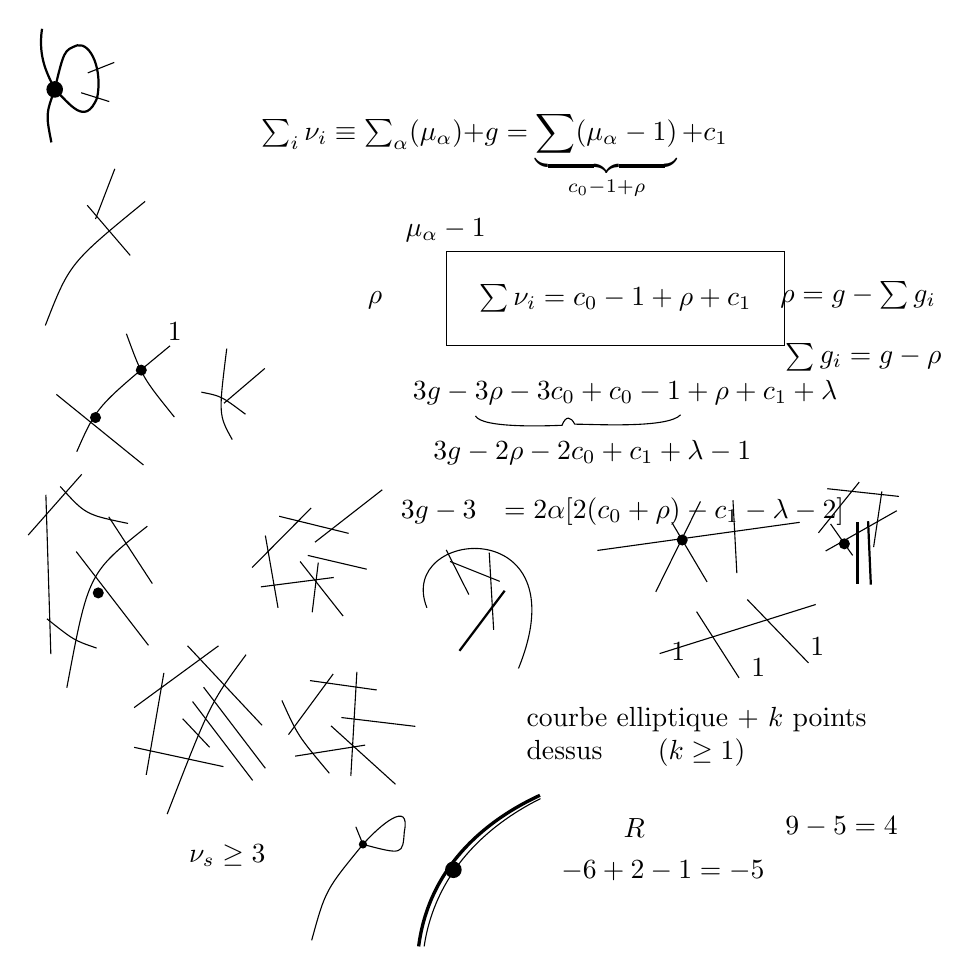
\begin{tikzpicture}[x=.007cm,y=-.007cm]
\draw[thick] (80,515)..controls (72,570) and (92,600)..(103,625)..controls (130,650) and (158,694)..(180,640)..controls (190,590) and (169,540)..(144,545)..controls (120,554)..(103,625)..controls (87,670)..(97,721);
\fill (103,625) circle (3pt);\draw (163,595)--(211,576);\draw (151,631)--(202,647);
\draw (86,1053)..controls (130,940)..(267,828);\draw (162,835)--(240,926);\draw (177,860)--(212,769);
\node[anchor=west] at (460,745) {$\sum_i\nu_i\equiv\sum_\alpha(\mu_\alpha)\deleted{\unsure{+g}}=\underbrace{\sum(\mu_\alpha-1)}_{c_0-1+\rho}+c_1$};
\node at (812,881) {$\mu_\alpha-1$};
\node at (684,1008) {$\deleted{\unsure{\rho}}$};
\node[draw,inner sep=12pt] at (1120,1004) {$\sum\nu_i=c_0-1+\rho+c_1$};
\node at (1560,998) {$\rho=g-\sum g_i$};\node at (1570,1110) {$\sum g_i=g-\rho$};
\draw (143,1282)..controls (179,1200)..(312,1090);\draw (106,1178)--(264,1306);\draw (233,1068)..controls (262,1147)..(320,1219);\fill (177,1220) circle (2pt);\fill (260,1134) circle (2pt);\node at (321,1065) {$1$};
\draw (415,1095)..controls (400,1215)..(425,1260);\draw (369,1174)..controls (405,1181)..(449,1214);\draw (410,1194)--(484,1131);
\node[anchor=west] at (735,1175) {$3g-3\rho-\unsure{3c_0}+\deleted{c_0}-1+\rho+c_1+\lambda$};
\draw (866,1217)..controls (878,1240) and (998,1235)..(1023,1234)..controls (1030,1216) and (1039,1218)..(1046,1232)..controls (1082,1232) and (1215,1240)..(1238,1215);
\node[anchor=west] at (772,1284) {$3g-2\rho-2c_0+c_1+\lambda-1$};
\node[anchor=west] at (713,1390) {$3g-3\quad\deleted{\unsure{=2\alpha}}[2(c_0+\rho)-c_1-\lambda-2]$};
\draw (55,1433)--(152,1323);\draw (113,1345)..controls (159,1396)..(236,1412);\draw (87,1360)--(96,1649);\draw (201,1400)--(280,1521);\draw (271,1417)..controls (164,1502)..(125,1710);\draw (142,1463)--(273,1633);\draw (89,1585)..controls (138,1624)..(179,1638);\fill (182,1538) circle (2pt);
\draw (461,1492)--(568,1384);\draw (510,1399)--(636,1430);\draw (575,1446)--(697,1351);\draw (485,1434)--(508,1565);\draw (562,1470)--(669,1495);\draw (477,1527)--(609,1510);\draw (548,1481)--(626,1580);\draw (581,1483)--(570,1573);
\draw (813,1460)--(854,1541);\draw (820,1481)--(910,1517);\draw (891,1465)--(899,1605);\draw[thick] (837,1643)--(919,1534);\draw (778,1565)..controls (720,1420) and (1060,1390)..(944,1675);
\draw (1087,1461)--(1454,1410);\draw (1193,1536)--(1274,1372);\draw (1222,1410)--(1286,1518);\draw (1333,1370)--(1340,1502);\fill (1241,1442) circle (2pt);
\draw (1488,1429)--(1562,1337);\draw (1504,1349)--(1634,1363);\draw (1510,1413)--(1550,1470);\draw (1501,1462)--(1630,1389);\draw (1603,1354)--(1588,1455);\draw[very thick] (1559,1410)--(1559,1522);\draw[thick] (1578,1408)--(1583,1523);\fill (1535,1449) circle (2pt);
\draw (1200,1648)--(1483,1559);\draw (1267,1572)--(1344,1692);\draw (1359,1550)--(1470,1665);\node at (1234,1645) {$1$};\node at (1379,1674) {$1$};\node at (1486,1636) {$1$};
\draw (247,1746)--(400,1634);\draw (301,1683)--(269,1868);\draw (344,1634)--(479,1778);\draw (450,1650)..controls (385,1738)..(307,1939);\draw (373,1709)--(485,1856);\draw (353,1735)--(462,1878);\draw (335,1766)--(384,1818);\draw (247,1818)--(409,1853);
\draw (527,1795)--(608,1685);\draw (566,1697)--(687,1714);\draw (651,1681)--(640,1870);\draw (515,1733)..controls (544,1797)..(601,1865);\draw (623,1764)--(757,1780);\draw (539,1834)--(666,1814);\draw (604,1779)--(721,1885);
\node[align=left] at (1267,1799) {courbe elliptique $+\ k$ points\\dessus\qquad$(k\geq1)$};
\node at (416,2015) {$\nu_s\geq3$};
\draw (569,2168)..controls (594,2077)..(662,1994)..controls (692,1960) and (749,1911)..(737,1971)..controls (734,2013)..(662,1994)--(649,1962);\fill (662,1994) circle (1.5pt);
\draw[very thick] (763,2179)..controls (781,2039) and (879,1953)..(983,1905);\draw (773,2179)..controls (792,2050) and (881,1962)..(984,1911);\fill (826,2040) circle (3pt);
\node at (1154,1965) {$\unsure{\mathbb R}$};\node at (1530,1962) {$9-5=4$};\node at (1206,2041) {$-6+2-1=-5$};
\end{tikzpicture}}

\scanpage{156}
% archive foliation: 155
\begin{center}41\end{center}
$\unsure{\mathfrak M|\mathcal M}(V)\cong\unsure{\mathfrak M|\mathcal M}(V*)$, we infer from the proposition \unsure{1)|i)} that $\widetilde\Phi$ induces an isomorphism $\unsure{\mathfrak M|\mathcal M}(\widetilde V)\cong\unsure{\mathfrak M|\mathcal M}(V*)$.

The inverse mapping $\widetilde\Phi^{-1}$ has possibly a finite number of fundamental points and branch curves and, except for these \uline{singular points}, $\widetilde\Phi^{-1}$ is locally bi-regular. Hence, for any general point $\mathfrak p*$ on $V*$, the inverse image $\widetilde\Phi^{-1}(\mathfrak p*)$ consists of a finite number of points and the number $m$ of these points is independent of $\mathfrak p*$. Now we show that $m=1$. Let $D_h^*$ be the section of $V*$ cut out by a general hypersurface of order $h$ containing no fundamental point of $\widetilde\Phi^{-1}$ and set $D_h=\widetilde\Phi^{-1}(D_h^*)$. Then, since $\widetilde\Phi$ induces the isomorphism $\unsure{\mathfrak M|\mathcal M}(\widetilde V)\cong\unsure{\mathfrak M|\mathcal M}(V*)$, \uline{the complete linear system} $|D_h|$ \uline{on} $\widetilde V$ \uline{and the complete linear system} $|D_h^*|$ \uline{on} $V*$ \uline{have the same dimension}. For sufficiently large $h$, we infer from the theorem of Riemann-Roch (2.10) and Theorem 2.4 that
\[
\dim|D_h^*|=\frac12(D_h^{*2})-\frac12(K*D_h^*)+\chi(V*)-1,
\]
where $K*$ is the canonical bundle on $V*$. Setting $2a=(D_1^{*2})$, $2b*=(K*D_1^*)$, we get therefore
\[
\dim|D_h^*|=ah^2-b*h+\chi(V*)-1.
\]
On the other hand, we get, using (2.10),
\[
\dim|D_h|\geqq\frac12(D_h^2)-\frac12(KD_h)+\chi(\widetilde V)-1-i(D_h).
\]
The general member $D_h^*$ of $|D_h^*|$ is an irreducible non-singular curve on $V*$. Let $D_h^{*\prime}$ be another general member of $|D_h^*|$ and

\scanpage{157}
% archive foliation: 156
\begin{flushright}
\unsure{Foncteurs|Foncteur} de Picard,\\
Diviseurs ...
\end{flushright}

\scanpage{158}
% archive foliation: 157
$X$ schéma \uline{Steinien} sur $S$

\deleted{\unsure{Soit}} Soit $\uline L$ inversible\inserted{très ample} sur $X$, tel que $f_*(\uline L)\inserted{=E}$ [soit libre de rang $N$]\inserted{tel que $i:X-\mathrm P(\unsure{E})$}
\margin{\unsure{inutile?}}
\margin{\unsure{sens ordinaire}}
\margin{$A_1$}
Équivalence

(i) Donner une base de $E=f_*(\uline L)$ i.e. un \uline{isom.} $\uline O_S^N\simeq\unsure{E}$

(ii) Donner un isom. $\varphi:\mathrm P_S^N\xrightarrow{\sim}\mathrm P(E\deleted{\unsure{L\to E}})$, $\oplus$ un isom.
$(\varphi^{-1}i)^*(\uline O(1))\simeq\uline L$

(iii) Donner un \deleted{\unsure{immersion}} morphisme
\[
j:X-\mathrm P_S^N
\]
$\oplus$ un isomorphisme $\alpha:j^*(\uline O(1))\simeq\uline L$
tel que l'hom canonique
\[
q_*(\uline O(1))\longrightarrow f_*(\uline L)=E
\]
soit un isom. [condition qui ne dépend pas du choix de $\alpha$]

\margin{\unsure{Dans la définition de spécial, faire attention qu'on exige que le changement de base donne un} \uline{morphisme spécial}.
\uuline{N.} $\unsure{f'_*f'^*(\uline L)}\uuline{\unsure{\simeq}}\unsure{N'\otimes_A A'}$}
\margin{Compatibles aux \unsure{deux} \unsure{opérations de $\Pi(g^*)$} et localisation.}

Équivalences

(i) Donner une \deleted{base}\inserted{section} du faisceau des germes de bases de $E$ modulo $\uline O_S^*$

(ii) Donner un isom. \unsure{$1$}
\[
\varphi:\deleted{\unsure{X}}\mathrm P_S^N-\mathrm P(E)
\]
(iii) Donner un morphisme
\[
j:X\longrightarrow P
\]
tel que

$1^\circ)$ $j^*(\uline O(1))\underset S\simeq\uline L$ \uuline{relativement à $S$}

$2^\circ)$ L'hom. $\underbrace{q_*(\uline O(1))\xrightarrow{\sim}f_*(j^*(\uline O(1)))\ \text{un isom.}}_{\text{morphisme spécial}}$

\scanpage{159}
% archive foliation: 158
Comme A est noethérien, il en est de même de $A'=A\{T_1,\ldots,T_r\}$ (7.5.4), donc $c)$ implique que B est noethérien; comme $\mathfrak J'=\mathfrak JA'$ est un voisinage ouvert de 0 dans $A'$ tel que les $\mathfrak J'^n$ forment un système fondamental de voisinages de 0, les images $\mathfrak J^nB$ des $\mathfrak J'^n$ forment un système fondamental de voisinages de 0 dans B, et comme on sait que B est séparé et complet, B est un anneau $\unsure{\mathrm J|\mathfrak J}B$-adique. Enfin, $B/\mathfrak JB$ est une algèbre (sur $A/\mathfrak J$) quotient de $A'/\mathfrak JA'=(A/\mathfrak J)[T_1,\ldots,T_r]$, donc est de type fini, ce qui achève de prouver que $c)$ entraîne $a)$.

Si B est $\mathfrak JB$-adique et noethérien, B est isomorphe à $\varprojlim B_n$, où $B_n=B/\mathfrak J^{n+1}B$ (7.2.11), et $\mathfrak JB/\mathfrak J^2B$ est un module de type fini sur $B/\mathfrak JB$. Soit $(a_j)_{1\leq j\leq s}$ un système de générateurs du $(B/\mathfrak JB)$-module $\mathfrak JB/\mathfrak J^2B$, et $(c_i)_{1\leq i\leq r}$ un système d'éléments de $B/\mathfrak J^2B$ dont les classes mod. $\mathfrak JB/\mathfrak J^2B$ forment un système de générateurs de la $(A/\mathfrak J)$-algèbre $B/\mathfrak JB$; on voit aussitôt que les $c_i a_j$ forment un système de générateurs de la $(A/\mathfrak J^2)$-algèbre $B/\mathfrak J^2B$, donc $a)$ implique $b)$.

Reste à prouver que $b)$ entraîne $c)$. L'hypothèse entraîne que $B_1$ est un anneau noethérien, et comme $B_1=B_2/\mathfrak J^2B_2$, on a $\mathfrak J^2B_1=0$, donc $\mathfrak JB_1=\mathfrak JB_1/\mathfrak J^2B_1$ est un $B_0$-module de type fini. Les conditions de (7.2.7) sont donc vérifiées par le système projectif $(B_n)$ et B est un anneau $\mathfrak JB$-adique. Soit $(c_i)_{1\leq i\leq r}$ un système fini d'éléments de B dont les classes mod. $\mathfrak J^2B$ engendrent la $(A/\mathfrak J^2)$-algèbre $B/\mathfrak J^2B$ (isomorphe à $B_1$).
\margin{\unsure{définition insuffisante} il faut aussi que les $c_i\in JB$ engendrent $JB/J^2B$ !}
Il existe donc un A-homomorphisme continu $u$ de $A'=A\{T_1,\ldots,T_r\}$ dans B qui se réduit à $\varphi$ dans A et est tel que $u(T_i)=c_i$ pour $1\leq i\leq r$ (7.5.3); si nous prouvons que $u$ est \textit{surjectif}, $c)$ sera établi, car de $u(A')=B$ on déduira $u(\mathfrak J^nA')=\mathfrak J^nB$, autrement dit $u$ sera un morphisme strict d'anneaux topologiques et B sera donc isomorphe à un quotient de $A'$ par un idéal fermé. Or, comme B est complet pour la topologie $\mathfrak JB$-adique, il suffit ([1], p. 18-07) de montrer que l'homomorphisme $\mathrm{grad}(A')\to\mathrm{grad}(B)$ déduit canoniquement de $u$ pour les filtrations $\mathfrak J$-adiques sur $A'$ et B, est surjectif. Mais par définition, les homomorphismes $A'/\mathfrak JA'\to B/\mathfrak JB$ et \uline{$\mathfrak JA'/\mathfrak J^2A'\to\mathfrak JB/\mathfrak J^2B$ déduits de $u$ sont surjectifs}; par récurrence sur $n$, on en déduit aussitôt qu'il en est de même de $\mathfrak JA'/\mathfrak J^nA'\to\mathfrak JB/\mathfrak J^nB$, et \textit{a fortiori} de $\mathfrak J^nA'/\mathfrak J^{n+1}A'\to\mathfrak J^nB/\mathfrak J^{n+1}B$, ce qui achève la démonstration.
\margin{!}

\textbf{7.6.} \textit{Anneaux complets de fractions.}

\textbf{(7.6.1)} Soient A un anneau linéairement topologisé, $(\mathfrak J_\lambda)$ un système fondamental de voisinages de 0 dans A formé d'idéaux, S une partie multiplicative de A. Soit $u_\lambda$ l'homomorphisme canonique $A\to A_\lambda=A/\mathfrak J_\lambda$, et pour $\mathfrak J_\mu\subset\mathfrak J_\lambda$, soit $u_{\lambda\mu}$ l'homomorphisme canonique $A_\mu\to A_\lambda$. Posons $S_\lambda=u_\lambda(S)$, de sorte que $u_{\lambda\mu}(S_\mu)=S_\lambda$. Les $u_{\lambda\mu}$ donnent canoniquement des homomorphismes surjectifs $S_\mu^{-1}A_\mu\to S_\lambda^{-1}A_\lambda$, pour lesquels ces anneaux forment un système projectif; désignons par $A\{S^{-1}\}$ la limite projective de ce système. Cette définition ne dépend pas du système fondamental de voisinages $(\mathfrak J_\lambda)$ choisi; en effet:

\textit{Proposition} \textbf{(7.6.2).} --- \textit{L'anneau $A\{S^{-1}\}$ est topologiquement isomorphe au séparé complété de l'anneau $S^{-1}A$ pour la topologie dont un système fondamental de voisinages de 0 est formé des $S^{-1}\mathfrak J_\lambda$.}

\scanpage{160}
% archive foliation: 159
On ne suppose plus donné de $\unsure{\uline L|E}$

$A'')$ Équivalence des deux données suivantes

(i) Une $S$-classe $\xi$ de faisceaux inversibles sur $S$,\inserted{qui est \uline{\unsure{amplissime}}} et un isom
\[
\varphi:\mathrm P^N_{\unsure{S|\xi}}\xrightarrow{\sim}P_\xi
\]
(ii) Une Donnée d'un morphisme
\[
j:X\longrightarrow\mathrm P_S^N
\]
tel que \deleted{$\unsure{j^*(\uline L)}$}
\[
q_*(\uline O(1))\longrightarrow f_*(j^*(\uline O(1)))
\]
soit un isomorphisme
\margin{\uline{morphisme spécial}\quad ou \unsure{projectif}}
\margin{Attention, $2$\quad\inserted{spécial,}
\diagram{\begin{tikzcd}[row sep=large]
\uline L\ \text{\unsure{magnifique|amplissime} sur }X/S+\text{trivialisation projective}
\arrow[d]\arrow[ddd,bend right=65,"\unsure{isom induit par un homoth. identique}"']\\
S\text{-classe }\xi\text{ sur }S,+\text{trivialisation projective}\arrow[d,equal]\\
\text{Morphisme spécial }X-\mathrm P_S^N\arrow[d]\\
\uline L'\ \text{\unsure{magnifique|amplissime} spécial sur }X,\text{ et trivialisation projective}
\end{tikzcd}}
$\#$
}
\deleted{\unsure{Les données}\illegible{2}}

$A''')$ Équivalence entre les données

(i) Une $S$-classe de faisceaux sur $X$ \deleted{\unsure{très ample}\illegible{1}\ ``spécial''}\inserted{\unsure{amplissime} et spécial}

(ii) Un fibré de Brauer-Severi sur $S$, associé à un fibré \uline{principal} $\mathcal P$ de groupe $GP\deleted{\unsure{L}}(N)$
$+$ morphisme \uline{spécial}
\[
j:X_{\unsure{\mathcal P}}-P^N_{\unsure{\mathcal P}\deleted{\unsure{\mathrm{Pic}}}}
\]
\deleted{\unsure{le morphisme}}\inserted{ce morphisme étant \uline{covariant} pour $GP(N)$}

\margin{spécial $=$ \unsure{pour ch. fibre en dim} $0$, et les \unsure{points définissent un morphisme, vers un projectif entier, comme} \illegible{2} de \deleted{\unsure{dim.}}\inserted{\unsure{dim.}}\unsure{fibre} $N$}

Si on introduit $\unsure{\mathfrak J}\ \uuline{\mathrm{Hom}}_S(X,P^N)$, où $GP(N)$ opère,
le sous-schém. $\unsure{\mathcal J}:\uuline{\mathrm{Hom}}_S^{\mathrm{spéc}}(X,P^N)$
[cas $X$ \deleted{\unsure{propre}} projectif sur $S$ loc noeth], alors on voit que
$\deleted{GP}(N)$ opère \uline{sans pts fixes} sur $\uuline{\mathrm{Hom}}_S^{\mathrm{spéc}}(X,P^N)$,
et les structures $A'''$ sont

\margin{\unsure{pour les points géométriques}\illegible{3}\ \unsure{introduire} \uline{\unsure{projectif}}\ \unsure{de passage}\illegible{2}.
\unsure{le morphisme}\illegible{2}\ $\unsure{j^*(\uline O(1))}$ \unsure{est}\illegible{2}
\deleted{\unsure{fibre}} \unsure{sur les fibres}\illegible{2}\ $\unsure{\mu}$
\deleted{$\unsure{\mathrm{Hom}_{\mathcal P}(X,\mathrm P^N)}$}\ $\unsure{\mathrm{Hom}}$}

\scanpage{161}
% archive foliation: 160
section des idéaux premiers $\mathfrak j_y$ pour $y\in Y$. Il est clair que la relation $Y\subset Y'$ entraîne $\mathfrak j(Y)\supset\mathfrak j(Y')$ et que l'on a
\[
\mathfrak j(\bigcup_\lambda Y_\lambda)=\bigcap_\lambda\mathfrak j(Y_\lambda)\tag{1.1.3.1}
\]
pour toute famille $(Y_\lambda)$ de parties de X.
\inserted{Enfin $\boxed{\mathfrak j(\{x\})=\mathfrak j_x}$}
\margin{(sert pour 1.1.7. !)}

\textit{Proposition} \textbf{(1.1.4).} --- (i) \textit{Pour toute partie E de A, on a $\mathfrak j(V(E))=\mathrm r(E)$.}

(ii) \textit{Pour toute partie Y de X, $V(\mathfrak j(Y))=\overline Y$, adhérence de Y dans X.}

(i) est conséquence immédiate des définitions et de (1.1.1.1); d'autre part, $V(\mathfrak j(Y))$ est fermé et contient Y; inversement, si $Y\subset V(E)$, on a $f(y)=0$ pour tout $f\in E$ et tout $y\in Y$, donc $E\subset\mathfrak j(Y)$, $V(E)\supset V(\mathfrak j(Y))$, ce qui prouve (ii).

\textit{Corollaire} \textbf{(1.1.5).} --- \textit{Les parties fermées de $X=\operatorname{Spec}(A)$ et les idéaux de A égaux à leurs racines (autrement dit les intersections d'idéaux premiers) se correspondent biunivoquement par les applications décroissantes $Y\to\mathfrak j(Y)$, $\mathfrak a\to V(\mathfrak a)$; à la réunion $Y_1\cup Y_2$ de deux parties fermées correspond $\mathfrak j(Y_1)\cap\mathfrak j(Y_2)$, et à l'intersection d'une famille quelconque $(Y_\lambda)$ de parties fermées correspond la racine de la somme des $\mathfrak j(Y_\lambda)$.}

\textit{Corollaire} \textbf{(1.1.6).} --- \textit{Si A est un anneau noethérien, $X=\operatorname{Spec}(A)$ est un espace noethérien..}

On notera que la réciproque de ce corollaire est inexacte, comme le montre l'exemple d'un anneau intègre non noethérien ayant un seul idéal premier $\ne\{0\}$, par exemple un anneau de valuation non discrète de rang 1.

Comme exemple d'anneau A dont le spectre n'est pas un espace noethérien, on peut signaler l'anneau $\mathcal C(Y)$ des fonctions continues numériques sur un espace compact infini Y; on sait qu'en tant qu'ensemble, Y s'identifie à l'ensemble des idéaux maximaux de A, et il est facile de voir que la topologie induite sur Y par celle de $X=\operatorname{Spec}(A)$ est la topologie initiale de Y. Comme Y n'est pas un espace noethérien, il en est donc de même de X.

\textit{Corollaire} \textbf{(1.1.7).} --- \textit{Pour tout $x\in X$, l'adhérence de $\{x\}$ est l'ensemble des $y\in X$ tels que $\mathfrak j_x\subset\mathfrak j_y$. Pour que $\{x\}$ soit fermé, il faut et il suffit que $\mathfrak j_x$ soit maximal.}

\textit{Corollaire} \textbf{(1.1.8).} --- \textit{L'espace $X=\operatorname{Spec}(A)$ est un espace de Kolmogoroff.}

En effet, si $x,y$ sont deux points distincts de X, on a, soit $\mathfrak j_x\not\subset\mathfrak j_y$, soit $\mathfrak j_y\not\subset\mathfrak j_x$, donc l'un des points $x,y$ n'appartient pas à l'adhérence de l'autre.

\textbf{(1.1.9)} D'après la prop. (1.1.\deleted{1}\inserted{2}, (iv)), pour deux éléments $f,g$ de A, on a
\[
D(fg)=D(f)\cap D(g)\tag{1.1.9.1}
\]
Notons aussi que la relation $D(f)=D(g)$ signifie, d'après la prop. (1.1.4, (i)) et la prop. (1.1.1, (v)) que $\mathrm r(f)=\mathrm r(g)$, ou encore que les idéaux premiers minimaux contenant $(f)$ et $(g)$ sont les mêmes; en particulier, il en est ainsi lorsque $f=ug$, où $u$ est inversible.

\textit{Proposition} \textbf{(1.1.10).} --- (i) \textit{Lorsque $f$ parcourt A, les ensembles $D(f)$ forment une base de la topologie de X.}

(ii) \textit{Pour tout $f\in A$, $D(f)$ est quasi compact.} \inserted{En particulier $X=D(1)$ est qu-cpt}

(i) Soit U un ensemble ouvert dans X; par définition, on a $U=X-V(E)$ où E est une partie de A, et $V(E)=\bigcap_{f\in E}V(f)$, d'où $U=\bigcup_{f\in E}D(f)$.

\scanpage{162}
% archive foliation: 161
\unsure{en correspondance avec les} $\mathcal P$ \unsure{principaux} sur $X$ de groupe $GP(N)$, et les $S$-\unsure{morphismes}
\diagram{\begin{tikzcd}
\mathcal P\arrow[r]&\unsure{\mathcal J|\mathcal I}
\end{tikzcd}}
qui sont compatibles avec les opérations de $GP(N)$.
\inserted{($GP(N)$ opère sur $\unsure{\mathcal J|\mathcal I}$ sans pts fixes ($=\uuline{\operatorname{Aut}_S}(X)$ \unsure{trivial}) \unsure{d'où} $\simeq$)}

Donc $\simeq\unsure{\mathcal J|\mathcal I}/GP(N)$ \unsure{existe, c'est un espace}

\deleted{\unsure{aux}} $S$-morphismes
\[
\unsure{\mathcal P|S}-\unsure{\mathcal J|\mathcal I}/GP(N)\qquad\ldots\ldots
\]
\margin{\unsure{traduire cela pour} $\unsure{\mathcal J'|\mathcal I'}=\uuline{\operatorname{Imm}_S^{\mathrm{sp}}}(X,\mathbf P^N)$ et les \unsure{fibres} \uline{amples ordinaires}}

\scanpage{163}
% archive foliation: 162
\margin{\uline{Nouveau fascicule}}

\begin{center}
\textsc{Chapitre Premier}

LE LANGAGE DES SCHÉMAS

\textbf{Sommaire}
\end{center}

\begin{tabular}{ll}
\S\ 1. & Schémas affines.\\
\S\ 2. & Préschémas et morphismes de préschémas.\\
\S\ 3. & Produits de préschémas.\\
\S\ 4. & Sous-préschémas et morphismes d'immersion.\\
\S\ 5. & Préschémas réduits; condition de séparation.\\
\S\ 6. & Conditions de finitude.\\
\S\ 7. & Applications rationnelles.\\
\S\ 8. & Les schémas de Chevalley.\\
\S\ 9. & Compléments sur les faisceaux quasi cohérents.\\
\S\ 10. & Schémas formels.
\end{tabular}

Les \S\S\ 1 à 8 ne font guère que développer un langage, celui qui sera utilisé dans toute la suite. Notons cependant que, conformément à l'esprit général de ce Traité, les \S\S\ 7 et 8 seront moins utilisés que les autres, et de façon moins essentielle; on n'a d'ailleurs parlé des schémas de Chevalley que pour faire le lien avec le langage de Chevalley [1] et Nagata [9]. Le \S\ 9 donne des définitions et résultats sur les faisceaux quasi cohérents, dont certains ne se bornent plus à une traduction en langage « géométrique » de notions connues d'Algèbre commutative, mais sont déjà de nature globale; ils seront indispensables, dès les chapitres suivants, dans l'étude globale des morphismes. Enfin, le \S\ 10 introduit une généralisation de la notion de schéma, qui nous servira d'intermédiaire au chapitre III pour formuler et démontrer de façon commode les résultats fondamentaux de l'étude cohomologique des morphismes propres; par ailleurs, signalons que la notion de schéma formel semble indispensable pour exprimer certains faits de la « théorie des modules » (problèmes de classification des variétés algébriques). Les résultats du \S\ 10 ne seront pas utilisés avant le \S\ 3 du chapitre III et il est recommandé d'en omettre la lecture jusque-là.

\scanpage{164}
% archive foliation: 163
\[
Y\subset X
\]
\diagram{\begin{tikzcd}[row sep=large,column sep=small]
Y\subset X\arrow[d,dash]&X\times\operatorname{Pic}\arrow[d] &\\
{}&\underset{p}{\operatorname{Pic}}&\underset{d}{\operatorname{Div}}\arrow[l]\\
\underline L^Y&&
\end{tikzcd}}

$\xi\in\underline H^0_f(\underline L^Y)$ \unsure{on a}
\diagram{\begin{tikzcd}[column sep=small]
0\arrow[r,dash]&\operatorname{Ker}\arrow[r,dash]&\underline H^0_f(\underline L^Y)^\vee\arrow[r]&\underline O_Y\arrow[r,dash]&0
\end{tikzcd}}
\diagram{\begin{tikzcd}[column sep=small]
0\arrow[r]&\underline O_S\arrow[r]&\underline H^0_f(\underline L)\arrow[r]&\underline H^0_f(\underline L|Y)
\end{tikzcd}}
\diagram{\begin{tikzcd}[column sep=small]
\underline J\underline L\arrow[r]&\underline L\arrow[r]&\underline L|Y\arrow[r]&0
\end{tikzcd}}\qquad $\underline L=\underline J^{-1}$
\diagram{\begin{tikzcd}[column sep=small]
0\arrow[r]&\underline O_X\arrow[r]&\underline L\arrow[r]&\underline L|Y\arrow[r]&0
\end{tikzcd}}
\diagram{\begin{tikzcd}[column sep=small,row sep=tiny]
0\arrow[r]&\underline O_S\arrow[r]&\underline H^0_f(\underline L)\arrow[r]&\underline H^0_f(\underline L|Y)\arrow[r]&\underline H^1_f(\underline O_X)\\
&&\text{\unsure{Tangent relatif}}&\text{Tangent}&\text{Tangent}\\
&&\text{de }\operatorname{Div}/\operatorname{Pic}&\operatorname{Div}/S&\operatorname{Pic}/S
\end{tikzcd}}
\diagram{\begin{tikzcd}[column sep=small]
{}\arrow[r]&\underline H^1_f(\underline L)\arrow[r]&\underline H^1_f(\underline L|Y)\arrow[r]&\underline H^{\unsure{1|2}}_f\underline O_X
\end{tikzcd}}
\margin{\unsure{son annulation universelle implique que} $\operatorname{Div}/\operatorname{Pic}$ \unsure{est lisse le long de la section envisagée}}
\margin{\unsure{son annulation universelle implique que} $\operatorname{Div}$ \unsure{est lisse} \illegible{3} \unsure{au point}}

\scanpage{165}
% archive foliation: 164
\begin{center}- 34 -\end{center}
\hfill n$^\circ$ 297

Soient A un anneau topologique séparé, E un A-module topologique séparé. Soit $\unsure{\widetilde E|\widehat E}$ le groupe additif complété du groupe topologique commutatif E (\S\ 3, n$^\circ$5, th.2). L'application Z-bilinéaire $(\lambda,x)\longrightarrow\lambda x$ du produit $A\times E$ des groupes additifs A,E dans le groupe additif E se prolonge par continuité en une application Z-bilinéaire de $\widehat A\times\widehat E$ dans $\widehat E$ (n$^\circ$5, th.1), que nous désignerons encore par $(\lambda,x)\longrightarrow\lambda x$. En vertu du principe de prolongement des identités, on a encore $\lambda(\mu x)=(\lambda\mu)x$ pour $\lambda\in\widehat A$, $\mu\in\widehat A$, $x\in\widehat E$; la loi externe $(\lambda,x)\longrightarrow\lambda x$ définit donc sur $\widehat E$ une structure de $\widehat A$-module compatible avec la topologie de $\widehat E$; si en outre A admet un élément unité 1, cet élément est aussi élément unité de $\widehat A$, et si E est un A-module unitaire, on a encore $1.x=x$ pour $x\in\widehat E$ par le principe de prolongement des identités. Nous dirons que le $\widehat A$-module topologique $\widehat E$ ainsi défini est le \uline{complété} du A-module topologique E.

Soit E un A-module topologique, A et E n'étant pas nécessairement séparés; soient N (resp. F) l'adhérence de $\{0\}$ dans A (resp. E); N est un idéal bilatère de A (n$^\circ$3; prop.6) et F un sous-A-module de E (n$^\circ$1, prop.1); en outre on a par continuité $\lambda x\in F$ lorsque $\lambda\in N$ ou $x\in F$. On en déduit aussitôt, par passage aux quotients une application $(\mathring\lambda,\mathring x)\longrightarrow\mathring\lambda\mathring x$ de $(A/N)\times(E/F)$ dans $E/F$, et on vérifie aussitôt (grâce à la prop.24 du \S\ 2, n$^\circ$9) que cette application est loi de composition externe d'une structure de $(A/N$-module topologique sur $E/F$. Si l'on pose $B=A/N$, $L=E/F$, on dit que le B-module L est le module séparé \uline{associé} à E; son complété $\widehat L$ est un $\widehat B$-module topologique, qu'on appelle le module \uline{complété séparé} de E.

\scanpage{166}
% archive foliation: 165
A K
\hfill\uline{Pseudomorphismes}

$X$ un préschéma

ouvert schématiquement dense $U$: si $X$ est le plus petit ss-préschéma fermé de $X$ \unsure{dominant|contenant} $U$ i.e. si $\overline U=X$ [lorsque $U\to X$ est quasi-compact cela implique que pour tout ouvert $V$, $U\cap V$ est schématiquement dense dans $X$ --- aussi est-ce \unsure{mieux comme} définition: \unsure{toute} \uline{\unsure{fonction|section}} de $\underline O_X$ sur un ouvert de $X$ nulle sur $U\cap V$ est nulle]
\margin{\unsure{définition équivalente}}

\deleted{\unsure{L'indépendance}}
Caractère local de la notion

$U$ schématiquement dense ds $X\Longleftrightarrow$ [si $X=\bigcup X_i$, les $X_i$ ouverts, les $U\cap X_i$ sch. denses dans les $X_i$]

$U$ schématiq. dense ds $X\Longrightarrow U$ schém. dense ds \unsure{des} $V$ q.c. $U\subset V\subset X$

Si $U,U'$ sont schém. denses, leur $U\cap U'$ l'est

[Soit $X$ et $Y$ sur $S$, \deleted{$\unsure{X|Y}$} $Y$ séparé sur $S$, \deleted{$X\Rightarrow$} $U$ schém. dense dans $X$. Si $f,g:X\to Y$ sont des $S$-morphismes tels que $f|U=g|U$

\deleted{\unsure{Quasi}}\inserted{Pseudo}-morphismes: classes d'équivalence d'\deleted{applications} morphismes définis sur des ouverts schématiquement denses, \unsure{aussi} $S$-morphismes. Pour un \unsure{pseudo}-morphisme dans un $S$-\unsure{pré}\uline{schéma}, il y a un domaine \inserted{(plus grand)} de définition.

\deleted{\unsure{le domaine} $\operatorname{Dom}(f|V)=$} $\operatorname{Dom}(f|V)=\operatorname{Dom}(f)\cap V$

\scanpage{167}
% archive foliation: 166
\uline{Ex} Si $X$ \deleted{\unsure{est intègre les}} \inserted{est \uline{réduit}, alors schématiquement dense $=$ dense} \deleted{\unsure{ouverts sont les ouverts non vides}}

pseudo-morphismes $=$ applications rationnelles

Pour tout ouvert $U$ de $X$, soit $F(U)$ l'ens des pseudo-$S$-morphismes de $U$ dans $Y$ ($S$-schéma fixé). Applications de restriction $F(U)\unsure{-|\to}F(V)$ si $U\supset V$. Cela \deleted{est} définit un \uline{faisceau} [grâce à la relation $\operatorname{Dom}(f_i|U_{ij})=\operatorname{Dom}(f_j|U_{ij})$], appelé \uline{faisceau des} \deleted{\unsure{quasi-morphismes}} \uline{pseudo-$S$-morphismes} de $X$ ds $Y$.

En particulier, on obtient ainsi le faisceau des pseudo-sections de $O_X$ (faisant $X=S$, $Y=X[t]$) qui est un faisceau d'anneaux $\supset\underline O_X$, en particulier un faisceau d'algèbres.

\deleted{\uline{Prop.} 0.1 Ce faisceau est quasi-cohérent.
\unsure{Il suffit pour} $X=\operatorname{Spec}(A)$.}

\scanpage{169}
% archive foliation: 168
\margin{(Diviseurs de \uline{fonctions}}
Soit $X$ une variété irréductible \uline{normale} déf/$k$

$K=k(X)$ le corps des fonctions rationnelles/$k$ sur $X$

Soit $V$ un \deleted{\unsure{hypersurface irréductible}} \inserted{diviseur premier déf.} sur $k$ sur $X$

Alors l'ensemble des $f\in K$ \uline{définies} en $V$ forment un anneau de valuation discrète, \deleted{$\unsure{O_V}$} $\underline O_{(V)}$.

En effet, c'est une \deleted{\illegible{1}} localité normale, dont la dimension de Krull est 1.

Soit $v_V$ la valuation \inserted{de $K$} associée à cet anneau de valuation de $K$. Appelons \uline{diviseur} \inserted{déf/$k$} sur $X$ toute comb. lin. formelle des diviseurs premiers sur \unsure{déf}/$k$. Posons, pour tout $f\in K$
\[
\operatorname{div}f=\sum_{\substack{V\,\mathrm{div.}\\\mathrm{pr}/k}}v_V(f).V
\]
Cette somme a un sens, car pour $f$ donné, il n'y a qu'un nb fini de termes non nuls; \deleted{\unsure{ceci étant}} pour le voir, on est ramené au cas \deleted{\unsure{normal}} affine, alors les diviseurs pr. déf/$k$ correspondent aux idéaux premiers non nuls minimaux de l'anneau normal noethérien $A=k[X]$, et la chose est bien connue.

\uline{Théorème} \deleted{$\unsure{f\in K}$ \illegible{3} \unsure{partout}} \inserted{$\operatorname{div}f\geq0.\Longleftrightarrow f$ est partout définie}

Car. résulte de la théorie des anneaux normaux;
\[
A=\bigcap A_{\mathfrak p}\qquad(\mathfrak p\text{ premiers minimaux})\quad\text{si }A\text{ est normal.}
\]
En effet, on est aussitôt ramené au cas affine, et $\operatorname{div}f\geq0\Longleftrightarrow f\in\bigcap A_{\mathfrak p}$.

\scanpage{170}
% archive foliation: 169
\uline{Corollaire 1} \deleted{Pour que $f$ soit définie en une sous-variété irréductible $Y$, il faut et il suffit que $Y$ ne soit contenue dans aucun $V$ tel que} \inserted{L'ens. des pts de $X$ où $f$ n'est pas définie est la réunion des supports des $V$ tels que} $v_V(f)<0$. C'est encore vrai si $f$ est une application rationnelle de $X$ dans une variété \uline{\unsure{affine}} ($X$ normal)

C'est par suite une sous-variété pure de dim $n-1$.

\deleted{\illegible{1}} N.B. Les résultats précédents valent sans changement essentiel si \deleted{\unsure{singulier}} l'ens des pts singuliers de $X$ est de dim $\leq n-2$.

\uline{Th.} Soit $X$ une variété \deleted{non singulière}\inserted{normale de dim $n$}, $Y$ une variété complète, $f:X-Y$ une application rationnelle. Alors l'ens. des pts où $f$ n'est pas définie est de dim $\leq n-2$.

\deleted{\unsure{On peut supposer} $X$}
Deux démonstrations

a) On peut supposer, en regardant le graphe de $f$, que $f$ est inverse d'un \uline{morphisme} birationnel $g:Y\to X$, et $g$ est \deleted{propre} \uline{propre}.

\uline{Lemme} Soit $X'$ l'ens des pts $x$ \deleted{\unsure{de}} tels que $g^{-1}(x)$ soit de dim $>0$, alors $X'$ est de dim $\leq n-2$, car sinon $g^{-1}(X')$ serait de dim $\geq(n-1)+1=n$, absurde. \deleted{Donc $g^{-1}(X)$} D'autre part, il résulte du Main Th. qu'en dessus de $\complement X'$, $g$ est un isom. birégulier, donc $g^{-1}$ est définie sur $\complement X'$. O.K.

N.B. Bien entendu, le th. se généralise aussi au cas où l'ens des singularités de $X$ est de dim $\leq n-2$.

\scanpage{171}
% archive foliation: 170
\margin{On suppose $X$ irréductible, $f$ dominante, ce qui est possible.}

b) Soit $V$ une hypersurface irréductible de $X$.

Pour voir que $f$ est définie en au moins un pt de $V$, \deleted{\unsure{il en}} i.e. $f$ ``définie en la localité $\underline O_{(V)}$'', il faut montrer qu'il existe une localité de $Y$ dominée par $\underline O_{(V)}$. Or cela résulte de la définition abstraite des variétés complètes, et du fait que $\underline O_{(V)}$ est un anneau de valuation.

\scanpage{173}
% archive foliation: 172
\uline{Le foncteur de Picard}
\margin{Faits élémentaires sur les classes de diviseurs, faisceaux inversibles, leurs propriétés etc}

Soit $X$ un $S$-préschéma, on pose
\[
\mathrm{Prépic}(X/S)=\deleted{H^1(X,\underline O_X^*)}\ \operatorname{Pic}(X\deleted{\unsure{/S}})=H^1(X,\underline O_X^*)
\]
\[
\underline{\underline{\mathrm{Prépic}}}_{X/S}(S')=\mathrm{Prépic}(X'/S')=H^1(X',\underline O_{X'}^*)
\quad\text{où }X'=X\times_S S'
\]
donc $\underline{\underline{\mathrm{Prépic}}}_{X/S}$ est bien un foncteur \uline{contravariant} sur les préschémas $S'$
\[
\mathrm{Prépic}'(X/S)=\Gamma(S,\underline H^1_{X/S}(\underline O_X^*))
\]
\[
\underline{\underline{\mathrm{Prépic}}}'_{X/S}(S')=\Gamma(S',\underline H^1_{X'/S'}(\underline O_{X'}^*))
\quad\text{où }X'=X\times_S S'
\]
On passe de $\underline{\underline{\mathrm{Prépic}}}$ à $\underline{\underline{\mathrm{Prépic}}}'$ en effectuant la descente par recouvrements ouverts.
\margin{expliciter les \unsure{objets}, \unsure{l'épimorphisme} $\operatorname{Pic}(X\deleted{/S})$ défini par $\operatorname{Pic}(X)\twoheadrightarrow\mathrm{Prépic}'(X/S)$}

\uline{Proposition 1} Supposons $\underline H^0_{X/S}(\underline O_X)=\underline O_S$. Alors on a un \deleted{isomorphisme}\inserted{monomorphisme} canonique
\[
\mathrm{Prépic}'(X/S)\longleftarrow\mathrm{Prépic}(X/S)/\operatorname{Pic}\mathrm{abs}(S)
\]
qui est un isomorphisme si $X/S$ a une section.

Résulte de l'assertion plus précise
\margin{mettre ce \deleted{corollaire} sous forme d'une suite exacte plutôt}

\uline{Corollaire 1} Le foncteur $\underline F\to\underline F\otimes_S X$ des faisceaux loc. libres de $S$ dans les faisceaux loc. libres de $X$ \deleted{définit} est \uline{pleinement} fidèle, l'image essentielle est formée des faisceaux loc. libres sur $X$ qui sont triviaux loc. en dessus de $\unsure{Y|S}$, le foncteur inverse sur ce domaine est le foncteur $\underline H^0_{X/S}$.
\margin{\unsure{val. pour une cond. plus forte} \illegible{2} \unsure{projection pleinement}}
\margin{\unsure{dire que le} \illegible{2} \unsure{est un} \illegible{1}}

\scanpage{174}
% archive foliation: 173
Il en résulte en effet que l'on a une suite exacte (en se bornant aux faisceaux inversibles)
\diagram{\begin{tikzcd}[column sep=small]
0\arrow[r]&\operatorname{Pic}(S)\arrow[r]&\operatorname{Pic}(X)\arrow[r]&\mathrm{Prépic}'(X/S)
\end{tikzcd}}
l'image \inserted{dernière} étant formée des sections de $\underline H^1_{X/S}(\underline O_X^*)$ qui sont dans l'image de $\underline H^1(\underline O_X^*)$ i.e. dont l'obstruction dans $H^2(S,\underline O_S^*)$ est nulle.
\margin{[lorsque $X/S$ a une section] \unsure{les hom sont définis en tous cas}, mais l'exactitude demande que $\underline H^0_{X/S}(\underline O_X)=\underline O_S$}

[N.B. le début de la suite exacte n'est que la suite exacte de bord de la suite spectrale de Leray
\diagram{\begin{tikzcd}[column sep=small]
0\arrow[r]&H^1(S,\underline H^0(\underline O_X^*))\arrow[r]&H^1(X,\underline O_X^*)\arrow[r]&H^0(S,\underline H^1(\underline O_X^*))\arrow[r]&H^2(S,\underline H^0(\underline O_X^*))\arrow[d]\\
&&&&H^2(X,\underline O_X^*)
\end{tikzcd}}
compte tenu que $\underline H^0(\underline O_X^*)=\underline O_S^*$]. S'il y a une section $\inserted{s}$ de $X/S$, alors on \deleted{\unsure{aura un bien inverse}} a un résultat plus complet

\uline{Corollaire 2} Soit $\underline C$ la catégorie des faisceaux inversibles $\underline L$ sur $X$ munis d'un \uline{isomorphisme} $\underline O_S\to s^*(\underline L)$. Alors \deleted{pour}\inserted{(i)} tout automorphisme d'un objet de $\underline C$ est trivial.

(ii) Pour \deleted{tout} tout élém$^t$ de $\mathrm{Prépic}(X/S)$ provient d'un $\underline L\in\underline C$, déterminé à isom. unique près.

\scanpage{175}
% archive foliation: 174
Pour prouver (ii), on considère un recouvrement de $S$ par des $U_i$ tels que $\xi$ soit défini par des $\underline L_i$ sur $X_i=X|U_i$, prenant les $U_i$ assez petits

\deleted{[voisinages de tout $\unsure{s}\in S$] \unsure{on peut supposer que}}

Remplaçant $\underline L_i$ par $\underline L_i\otimes_S s^*(\underline L_i)^{-1}$, on peut supposer donnés des isom
\diagram{\begin{tikzcd}
\underline O_S|U_i\arrow[r,"{\substack{\varphi_i\\\sim}}"]&s^*(\underline L_i).
\end{tikzcd}}
Dans $X_{ij}=X|U_i\cap U_j$, $\underline L_i$ et $\underline L_j$ sont \uuline{$U_{ij}$-équivalents}, donc il y a un isomorphisme \uline{unique} $\varphi_{ij}$ de $\underline L_i$ sur $\underline L_j$ compatible avec les $\varphi_i$. De l'unicité résulte que les $\varphi_{ij}$ satisfont les conditions de recollement, d'où le $\underline L$ cherché.
\margin{\unsure{Lemme 2 qui est à introduire} en tout cas, il faut \unsure{commencer avec les démonstrations à coups de (longs} \illegible{2} \unsure{éléments)}}

Question: donner une formulation cohomologique des raisonnements.

\deleted{\uline{Corollaire 2}}\inserted{\uline{Proposition 2}} On suppose encore $\underline H^0_{X/S}(\underline O_X)=\underline O_S$, et $X$ quasi-compact séparé sur $S$, donc la relation précédente satisfaite après extension plate de la base. Soit $S'\to S$ une extension fid. plate \inserted{\unsure{qu. cpt}} de la base. (i) Alors
\deleted{\unsure{(i)}}
\diagram{\begin{tikzcd}
\deleted{\unsure{\operatorname{Pic}}}\ \mathrm{Prépic}'(X/S)\arrow[r]&\mathrm{Prépic}'(X'/S')
\end{tikzcd}}
est injectif. (ii) Si $X/S$ a \uline{localement} \uline{sur $S$} une section, alors la suite d'applications

\scanpage{176}
% archive foliation: 175
\deleted{$\unsure{0}$}
\diagram{\begin{tikzcd}
\mathrm{Prépic}'(X/S)\arrow[r]&\mathrm{Prépic}'(X'/S')\arrow[r,shift left=.5ex]\arrow[r,shift right=.5ex]&\mathrm{Prépic}'(X''/S'')
\end{tikzcd}}
[où $S''=S'\times_S S'$] est exacte \deleted{\unsure{i.e. le} \illegible{2} \unsure{dans}}
\deleted{$\underline{\underline{\mathrm{Prépic}}}_{X/S}$}

\deleted{\unsure{Soit}} En effet, le point (i) est encore une conséquence immédiate du

\uline{Corollaire 1} dans les conditions de Prop. 1)
\margin{($X$ supposé \unsure{q.c. qs} sur $S$)}

[Corollaire 1, soit $S'\to S$ une extension fid. plate \inserted{et q. cpte} de la base. Soit $\underline E$ faisceau \deleted{inversible}\inserted{loc. libre} sur $X$. Pour qu'il soit isomorphe à l'image inverse d'un faisceau loc libre \deleted{[\unsure{représenté}]} sur $S$, il faut que $\underline E'$ soit isomorphe à l'image inverse d'un faisceau loc libre sur $S$.

En effet, il faut exprimer que $f_*(\underline E)$ est loc. libre et \deleted{$\unsure{\xi}$} $f^*f_*(\underline E)-\underline E$ (appl \unsure{naturelle|canonique}) un isom. Or
\[
f_*(\underline E)'=f_*(\underline E')
\]
\margin{extension plate}
on est ramené à des assertions élémentaires, de stabilité de propriétés par extensions fid. plates (chap IV)

\scanpage{177}
% archive foliation: 176
Pour prouver (ii), on est ramené à prouver que tout élément de $\mathrm{Prépic}'(X'/S')$ dont les images sont les mêmes, provient d'une classe de $\mathrm{Prépic}'(X/S)$. À cause de l'unicité, on voit que c'est local sur $S$, on peut donc supposer qu'on a une section de $X$ sur $S$. On peut alors identifier les \deleted{\unsure{classes}}\inserted{élts} de $\mathrm{Prépic}(X/S)$ à des faisceaux inversibles \inserted{(à isom. unique près)} sur $X$ à section marquée sur $S$, ce qui permet d'appliquer la théorie de la descente \uline{fid. plate}.

\uline{Corollaire 2} Même conclusion que Prop 1. (ii) pour descendre des \uline{faisceaux} sur $X$.

\uline{Corollaire 3} Supposons que la relation $\underline H^0_{X/S}(\underline O_X)=\underline O_S$ reste vraie par tte extension de la base (i.e., $X$ coh. plat sur $S$ en dim 0, et $\underline H^0_{X/S}(\underline O_X)=\underline O_S$), \inserted{et $X/S$ a localement une section} Alors le foncteur $\underline{\underline{\mathrm{Prépic}}}'_{X/S}$ est compatible [= \unsure{ex. et pour}] avec la descente fidèlement plate quasi-compacte.

\scanpage{178}
% archive foliation: 177
\deleted{\unsure{Proposition 3}}

$\underline{\underline{\operatorname{Pic}}}_{X/S}=$ enveloppe exacte de $\underline{\underline{\mathrm{Prépic}}}_{X/S}$ (ou $\underline{\underline{\mathrm{Prépic}}}'_{X/S}$) pour la descente fid. plate quasi-compacte

[Il y a un ennui, car un \uline{recouvrement} ouvert d'un préschéma non quasi-cpt. n'est en général pas majoré par un morphisme fid. plat qu. cpt. Il faut donc dire au lieu de fid. plat qu. cpt: \deleted{fid plat séparé} \deleted{localisation} \uline{morphismes de localisation fidèlement plats}]

Donc on a des morphismes fonctoriels
\diagram{\begin{tikzcd}
\underline{\underline{\mathrm{Prépic}}}_{X/S}\arrow[r,"\alpha"]&\underline{\underline{\mathrm{Prépic}}}'_{X/S}\arrow[r,"\beta"]&\underline{\underline{\operatorname{Pic}}}_{X/S}
\end{tikzcd}}
Le premier morphisme n'est pas injectif en général [son noyau, si $\underline H^0_{X/S}(\underline O_X)=\underline O_S$, et si cela reste vrai par changement de base] est le foncteur $\underline{\underline{\operatorname{Pic}}}$ (absolu) en vertu de prop. 1, (i), \inserted{Il est surjectif} si on suppose en plus de la condition de [ ] que $X/S$ a une section. \deleted{$\unsure{\beta}$ \illegible{3}}
\margin{(\unsure{qui est non représentable par un schéma})}

\scanpage{179}
% archive foliation: 178
D'autre part $\beta$ est un mono. sous \unsure{les hypothèses|l'hypothèse} $\underline H^0_{X/S}(\underline O_X)=\underline O_S$ ``universelle''; et il est surjectif donc bijectif si on suppose \uline{de plus} que \deleted{$\unsure{\operatorname{Pic}}$} $X$ a localement une section sur $S$.

\uline{Exemple} où $\beta$ n'est pas surjectif: variété de \unsure{Séveri}-Brauer non triviale sur un corps .... On verra qu'il y a une obstruction à la surjectivité de $\beta$, à valeurs dans un $H^2(S,\mathbf G_m)$ .....

\uline{Remarque}

On voit donc que le foncteur \uuline{Prépic} n'est pas représentable \deleted{en général, \unsure{que dans un}} \inserted{sauf dans des cas} \deleted{\unsure{peu}} triviaux sans intérêt; $\mathrm{Prépic}'_{X/S}$ ne peut être représentable que si $\beta$ est un isom et si $\underline{\underline{\operatorname{Pic}}}_{X/S}$ est représentable, \deleted{\unsure{(que si} $\unsure{\beta}$} [ce qui est pratiquement lié à des conditions comme celles déjà envisagées, à savoir l'existence d'une section de $X$ sur $S$]. Quant à $\underline{\underline{\operatorname{Pic}}}_{X/S}$, il est représentable dans des cas généraux importants qui seront étudiés par la suite. C'est \unsure{peut être} le plus \unsure{important pour notre propos}.
